\appendix
\section{Specifica dei test}
\subsection{Test di validazione}
Questo tipo di test verrà utilizzato durante l'attività di collaudo del prodotto finale così da accertare che esso soddisfi le richieste del committente. Per ogni test viene specificato il proprio codice univoco, il codice identificativo del requisito ad esso associato, la descrizione e lo stato di implementazione attuale. 

	\begin{longtable}{|>{\centering\arraybackslash}m{1.6cm}|>{\centering\arraybackslash}m{6.41cm}|>{\centering\arraybackslash}m{3.1cm} | >{\centering\arraybackslash}m{2.6cm}|}		
		\rowcolor{LightBlue}
		\textbf{\textcolor{white}{Codice}}
		& \multicolumn{1}{|c|}{\textbf{\textcolor{white}{ Descrizione}}}
		& \textbf{\textcolor{white}{Esito}} & \textbf{\textcolor{white}{Requisito associato}}\\
		TV-RO1 & L'utente non riconosciuto vuole registrarsi alla piattaforma come allievo, creando un account personale. All'utente è richiesto di:
		\begin{itemize}
			\item Raggiungere la pagina di registrazione;
			\item Inserire i dati richiesti quali:
				\begin{itemize}
				 	\item nome;
				 	\item cognome;
				 	\item username;
				 	\item email;
				 	\item password;
				 	\item nome della scuola di appartenenza;
				 	\item città sede della scuola di appartenenza;
				\end{itemize}
			\item Confermare la registrazione.
		\end{itemize} & Non implementato & ROF1 \\ \hline
		\rowcolor{LightGray}
		TV-RO2 & L'utente non riconosciuto vuole registrarsi alla piattaforma come insegnante, creando un account personale. All'utente è richiesto di:
		\begin{itemize}
			\item Raggiungere la pagina di registrazione;
			\item Inserire i dati richiesti quali:
				\begin{itemize}
				 	\item nome;
				 	\item cognome;
				 	\item username;
				 	\item email;
				 	\item password;
				 	\item nome della scuola di appartenenza;
				 	\item città sede della scuola di appartenenza;
				 	\item codice INPS;
				\end{itemize}
			\item Confermare la registrazione.
		\end{itemize} & Non implementato & ROF22 \\ \hline
		TV-RO3 & L'utente non riconosciuto vuole eseguire l'accesso alla piattaforma tramite le sue credenziali. All'utente è richiesto di: 
		\begin{itemize}
			\item Raggiungere la pagina di autenticazione;
			\item Inserire il proprio username e password;
			\item Confermare l'accesso.
		\end{itemize} & Non implementato 
		& ROF2 \\ \hline
		  \rowcolor{LightGray}
		TV-RD1 & L'utente vuole modificare i dati del proprio profilo personale. All'utente è richiesto di:
		\begin{itemize}
			\item Raggiungere la pagina di modifica dei dati dal profilo;
			\item Modificare una o più voci tra username, password, scuola e città;
			\item Confermare la modifica.
		\end{itemize}& Non implementato  & RDF1 \\ \hline
		TV-RD2 & Il  moderatore vuole verificare le credenziali di un utente che vuole registrarsi come insegnante. Al moderatore è richiesto di:
		\begin{itemize}
			\item Raggiungere la pagina di amministrazione della piattaforma;
			\item Visualizzare la lista degli utenti che richiedono i  ruolo di insegnante;
			\item Il moderatore seleziona uno degli utenti;
			\item Il moderatore accetta o rifiuta l'utente selezionato.
		\end{itemize}& Non implementato  & RDF2 \\ \hline
		  \rowcolor{LightGray}
		TV-RD3 & L'utente vuole registrarsi alla piattaforma. 
		\begin{itemize}
			\item L'utente inserisce delle credenziali errate;
			\item L'utente visualizza un messaggio di errore.
		\end{itemize}& Non implementato  & RDF3 \\ \hline
		TV-RO4 & L'utente vuole cercare degli esercizi sulla piattaforma. All'utente è richiesto di:
		\begin{itemize}
			\item Raggiungere la pagina di ricerca degli esercizi;
			\item Scrivere una frase o parte di essa nella barra di ricerca;
			\item Selezionare, eventualmente, dei filtri per la ricerca;
			\item Avviare la ricerca.
		\end{itemize}& Non implementato  & ROF3 RPF1 RPF2 RPF3 RPF4\\ \hline
		  \rowcolor{LightGray}
		TV-RD4 & L'allievo vuole visualizzare la lista delle classi a cui appartiene. All'allievo è richiesto di: 
		\begin{itemize}
			\item Accedere alla pagina dedicata al proprio profilo;
			\item Selezionare l'opzione "lista delle classi".
		\end{itemize}& Non implementato  & RDF4 \\ \hline
		TV-RP1 & Il moderatore vuole eliminare un utente iscritto alla piattaforma. Al moderatore è richiesto di: 
		\begin{itemize}
			\item Visualizzare la lista degli utenti iscritti nella piattaforma;
			\item Indicare uno o più utenti da eliminare;
			\item Confermare l'eliminazione degli utenti  selezionati.
		\end{itemize}& Non implementato  & RPF5 \\ \hline
		  \rowcolor{LightGray}
		TV-RP2 & L'insegnante vuole modificare una soluzione di un esercizio da lui fornita. All'insegnante è richiesto di: 
		\begin{itemize}
			\item Selezionare la lista degli esercizi da lui inseriti;
			\item Visualizzare la precedente soluzione;
			\item Modificare le classi grammaticali della precedente soluzione;
			\item Confermare la modifica.
		\end{itemize}& Non implementato  & RPF6 \\ \hline
		TV-RD5 & L'insegnante vuole visualizzare la lista degli esercizi da lui creati. All'insegnante è richiesto di: 
		\begin{itemize}
			\item Accedere all'area del suo profilo;
			\item Selezionare la voce "esercizi inseriti".
		\end{itemize}& Non implementato  & RDF5 \\ \hline
		  \rowcolor{LightGray}
		TV-RP3 & L'insegnante vuole eliminare una soluzione di un esercizio da lui fornita. All'insegnante è richiesto di:
		\begin{itemize}
			\item Visualizzare la lista degli esercizi da lui inseriti;
			\item Selezionare una o più soluzioni da eliminare;
			\item Confermare l'eliminazione
		\end{itemize}& Non implementato  & RPF7 \\ \hline
		TV-RO5 & L'insegnante vuole inserire un esercizio nel sistema. All'insegnante è richiesto di: 
		\begin{itemize}
			\item Raggiungere la pagina di inserimento di un nuovo esercizio;
			\item Inserire una frase;
			\item Inserire una soluzione;
			\item Specificare gli argomenti;
			\item Specificare la difficoltà;
			\item Specificare se la soluzione è pubblica o privata;
			\item Confermare l'inserimento.
		\end{itemize}& Non implementato  & ROF4 ROF6 RPF8 RPF9\\ \hline
		  \rowcolor{LightGray}
		TV-RO6 & L'utente vuole svolgere un esercizio da lui indicato. All'utente è richiesto di:
		\begin{itemize}
			\item Raggiungere la pagina per l'esecuzione degli esercizi;
			\item Inserire una frase da svolgere o selezionare un esercizio dal sistema;
			\item Compilare i campi;
			\item Confermare i dati inseriti;
			\item Visualizzare la soluzione.
		\end{itemize}& Non implementato  & ROF6 ROF7 ROF8\\ \hline
		TV-RD6 & L'allievo vuole visualizzare i dati relativi ai propri progressi. All'allievo è richiesto di:
		\begin{itemize}
			\item Accedere alla vista del proprio profilo;
			\item Visualizzare i dati relativi ai propri progressi.
		\end{itemize}& Non implementato  & RDF6 \\ \hline
		  \rowcolor{LightGray}
		TV-RD7 & Lo sviluppatore vuole visualizzare la lista delle annotazioni di una particolare frase. Allo sviluppatore è richiesto di: 
		\begin{itemize}
			\item Accedere all'area dati;
			\item Scrivere una frase o parte di essa all'interno della barra di ricerca;
			\item Selezionare eventualmente i filtri di ricerca;
			\item Confermare la ricerca.
		\end{itemize}& Non implementato  & RDF7 RDF8 RDF9 RDF10 RDF18 \\ \hline
		TV-RP4 & Lo sviluppatore vuole visualizzare i dati relativi ad una particolare annotazione. Allo sviluppatore è richiesto di:
		\begin{itemize}
			\item Visualizzare la lista delle annotazioni ricercate;
			\item Selezionare un'annotazione;
			\item Visualizzare data, utente e soluzione proposta.
		\end{itemize}& Non implementato  & RPF10 \\ \hline
		  \rowcolor{LightGray}
		TV-RP5 & Lo sviluppatore vuole visualizzare lo storico delle annotazioni. Allo sviluppatore è richiesto di:
		\begin{itemize}
			\item Visualizzare la lista delle annotazioni cercate;
			\item Selezionare la voce "vedi storico".
		\end{itemize}& Non implementato  & RPF11 \\ \hline
		TV-RP6 & Lo sviluppatore vuole ordinare la lista dei risultati ottenuti dalla ricerca. Allo sviluppatore è richiesto di: 
		\begin{itemize}
			\item Visualizzare la lista delle annotazioni ricercate;
			\item Scegliere un parametro secondo il quale ordinare i risultati;
			\item Confermare l'ordinamento scelto.
		\end{itemize}& Non implementato  & RPF12 \\ \hline
		  \rowcolor{LightGray}
		TV-RO6 & Lo sviluppatore vuole scaricare un file contenente i dati relativi agli esercizi ottenuti con la ricerca. Allo sviluppatore è richiesto di:
		\begin{itemize}
			\item Visualizzare la lista delle annotazioni ricercate;
			\item Richiedere il download dei dati;
			\item Scegliere il path per il salvataggio del file;
			\item Confermare ed eseguire il salvataggio.
		\end{itemize}& Non implementato  & ROF9 \\ \hline
		TV-RP7 & Lo sviluppatore vuole visualizzare le informazioni relative ad un dataset. Allo sviluppatore è richiesto di: 
		\begin{itemize}
			\item Visualizzare la lista delle annotazioni ricercate,
			contenente l'input della frase della fase di train del software di apprendimento automatico in base alla ricerca effettuata;
			\item Richiedere il download dei dati;
			\item Scegliere il path per il salvataggio del file;
			\item Confermare ed eseguire il salvataggio.
		\end{itemize}& Non implementato  & RPF13 \\ \hline
		  \rowcolor{LightGray}
		TV-RP8 & Lo sviluppatore vuole scaricare un modello. Allo sviluppatore è richiesto di:
		\begin{itemize}
			\item Visualizzare la lista dei modelli disponibili per l'applicazione;
			\item Selezionare un modello;
			\item Selezionare l'opzione "download";
			\item Scegliere il path per il salvataggio del file;
			\item Confermare ed eseguire il salvataggio.			
		\end{itemize}& Non implementato  & RPF14 \\ \hline
		
		TV-RP9 & Lo sviluppatore creare un modello alla piattaforma. Allo sviluppatore è richiesto di:
\begin{itemize}
 \item Selezionare la voce ”Aggiungi modello”;
 \item Inserire un file contenente il dataset;
 \item Confermare la creazione.
\end{itemize}& Non implementato  & RPF15 \\ \hline

		  \rowcolor{LightGray}
TV-RP10 & Il moderatore vuole eliminare un esercizio. Al moderatore è richiesto di:
\begin{itemize}
 \item Indicare gli esercizi da eliminare;
 \item Confermare l'eliminazione dell'esercizio.
\end{itemize}& Non implementato  & RPF16 \\ \hline

TV-RO7 & L'insegnante vuole creare una classe. All'insegnante è richiesto di:
\begin{itemize}
 \item Selezionare l'opzione "Crea classe";
 \item Assegnare un nome alla classe;
 \item Assegnare una descrizione alla classe;
 \item Confermare la creazione della classe.
\end{itemize}& Non implementato  & ROF10 \\ \hline

		  \rowcolor{LightGray}
TV-RO8 & L'insegnante vuole eliminare una classe. All'insegnante è richiesto di:
\begin{itemize}
 \item Cliccare sul pulsante di eliminazione della classe;
 \item Confermare l'eliminazione della classe.
\end{itemize}& Non implementato  & ROF11 \\ \hline

TV-RO9 & L'insegnante vuole aggiungere degli alunni ad una classe. All'insegnante è richiesto di:
\begin{itemize}
 \item Selezionare l'opzione "Aggiungi alunni";
 \item Visualizzare la lista di tutti gli alunni presenti sulla piattaforma;
 \item Scrivere l'username di un alunno, o una sua parte;
 \item Selezionare gli alunni da inserire;
 \item Confermare l'inserimento.
\end{itemize}& Non implementato  & ROF12, RPF17, RPF18 \\ \hline

		  \rowcolor{LightGray}
TV-RO10 & L'insegnante vuole assegnare degli esercizi ad una classe. All'insegnante è richiesto di:
\begin{itemize}
 \item Selezionare degli esercizi in lista da assegnare;
 \item Indicare la classe a cui assegnarli;
 \item Scrivere l'username di un alunno, o una sua parte;
 \item Confermare l'assegnazione.
\end{itemize} & Non implementato & ROF13 \\ \hline

TV-RP11 & L'insegnante vuole visualizzare i progressi di un alunno della classe. All'insegnante è richiesto di:
\begin{itemize}
 \item Selezionare uno studente;
 \item Visualizzare i grafici che riportano la media totale, la media per tipologia di
 esercizi e lo sviluppo della media nel tempo.
\end{itemize} & Non implementato & RPF19 \\ \hline
		
		  \rowcolor{LightGray}
	TV-RO11 & L'insegnante vuole eliminare un alunno dalla lista degli iscritti ad una classe. All'insegnante è richiesto di:
		\begin{itemize}
			\item Visualizzare la lista degli alunni della classe;
			\item Selezione l'allievo da rimuovere dalla classe;
			\item Confermare l'eliminazione.		
		\end{itemize} & Non implementato & ROF14 \\ \hline	
		
		TV-RO12 & L'insegnante vuole visualizzare la lista degli alunni iscritti ad una delle sue classi. All'insegnante è richiesto di:
		\begin{itemize}
			\item Accedere alla pagina di gestione delle proprie classi;
			\item Selezionare la voce "vedi alunni".		
		\end{itemize}& Non implementato  & ROF15 \\ \hline
		
		  \rowcolor{LightGray}
		TV-RO13 & L'insegnante vuole visualizzare la lista delle proprie classi. All'insegnante è richiesto di:
		\begin{itemize}
			\item Accedere alla pagina del proprio profilo;
			\item Selezionare la voce "vedi classi".		
		\end{itemize} & Non implementato & ROF16 \\ \hline
		
		TV-RD7 & L'allievo vuole annullare l'iscrizione ad una classe. Allo studente è richiesto di:
		\begin{itemize}
			\item Visualizzare la lista delle classi a cui appartiene;
			\item Selezionare l'opzione "disiscriviti".		
		\end{itemize}& Non implementato  & RDF11 \\ \hline
		
		  \rowcolor{LightGray}
		TV-RO14 & L'utente vuole autenticarsi alla piattaforma. 
		\begin{itemize}
			\item L'utente inserisce delle credenziali errate;
			\item L'utente visualizza un messaggio di errore.
		\end{itemize} & Non implementato & RDF17 \\ \hline
		
		TV-RO15 & L'utente vuole modificare le proprie credenziali. 
		\begin{itemize}
			\item L'utente inserisce delle credenziali errate;
			\item L'utente visualizza un messaggio di errore.
		\end{itemize} & Non implementato & RDF18 \\ \hline
		
		  \rowcolor{LightGray}
  TV-RP12 & L’allievo vuole selezionare un esercizio assegnato. All'allievo è richiesto di:
  \begin{itemize}
   \item Visualizzare le informazioni della classe indicata
   \item Selezionare un esercizio assegnato
  \end{itemize} & Non implementato & RPF28 \\ \hline

 TV-RO16 & L’insegnante vuole accedere all’area di inserimento nuovo esercizio. All'insegnante è richiesto di:
 \begin{itemize}
  \item Raggiungere la vista principale dell’applicazione.
  \item Selezionare la voce ”Inserisci esercizio”
 \end{itemize} & Non implementato & ROF23 \\ \hline
  \rowcolor{LightGray}
  TV-RD8 & L’utente riconosciuto vuole disconnettersi dalla piattaforma. All'utente è richiesto di:
  \begin{itemize}
   \item Selezionare l’opzione ”Logout” da qualsiasi vista dell'applicazione
  \end{itemize} & Non implementato & RDF25 \\ \hline
 
 TV-RP13 & Lo sviluppatore vuole visualizzare informazioni riguardanti i modelli disponibili nella piattaforma. Allo sviluppatore è richiesto:
 \begin{itemize}
  \item  Visualizzare la lista dei modelli disponibili per l’applicazione;
  \item Selezionare un modello
  \item Selezionare l’opzione ”Visualizza informazioni”
 \end{itemize} & Non implementato & RPF26 \\ \hline

\rowcolor{LightGray}
TV-RD9 & Lo sviluppatore vuole visualizzare la lista dei modelli disponibili.  Allo sviluppatore è richiesto di:

\begin{itemize}
 \item Raggiungere la vista dell’area dati.
 \item Selezionare la voce ”Lista dei modelli”
\end{itemize} & Non implementato & RDF23 \\ \hline

TV-RD10 & L’utente riconosciuto vuole accedere alla vista del proprio profilo personale. All'utente è richiesto di:
\begin{itemize}
  \item Raggiungere la vista principale dell'applicazione;
 \item Selezionare la voce ”Profilo personale”.
\end{itemize} & Non implementato & RDF22 \\ \hline

\rowcolor{LightGray}
TV-RD11 & L’insegnante vuole ricercare gli esercizi che ha inserito inserendo la frase o una parte di essa. All'insegnante è richiesto di:


\begin{itemize}
 \item Visualizzare la lista degli esercizi che ha inserito nella piattaforma;
 \item Scrivere nella barra di ricerca una frase o una sua parte.
\end{itemize} & Non implementato & RDF21 \\ \hline

TV-RP14 & Il moderatore vuole ricercare gli utenti inserendo l’username o una parte di esso. Al moderatore è richiesto di:
\begin{itemize}
 \item Visualizzare la lista degli utenti presenti nella piattaforma;
 \item Scrivere nella barra di ricerca una stringa.
\end{itemize} & Non implementato & RPF25 \\ \hline

		  \rowcolor{LightGray}
TV-RD12 & Il moderatore vuole visualizzare la lista degli utenti iscritti alla piattaforma. Al moderatore è richiesto di:
\begin{itemize}
 \item Raggiungere la vista di amministrazione dell’applicazione;
 \item Selezionare l’opzione ”Utenti”.
\end{itemize} & Non implementato & RDF20 \\ \hline

TV-RP15 & Il moderatore vuole ricercare gli esercizi inserendo la frase o una parte di essa. Al moderatore è richiesto di:

\begin{itemize}
 \item Raggiungere la lista degli esercizi inseriti nella piattaforma.
 \item Scrivere nella barra di ricerca una frase o una sua parte.
\end{itemize} & Non implementato & RPF24 \\ \hline

		  \rowcolor{LightGray}
TV-RD13 & Il moderatore vuole visualizzare la lista degli esercizi inseriti nella piattaforma. Al moderatore è richiesto di:

\begin{itemize}
 \item Raggiungere la vista di amministrazione dell’applicazione.
 \item Visualizzare la lista degli esercizi inseriti nella piattaforma.
\end{itemize} & Non implementato & RDF19 \\ \hline

TV-RD14 & L’insegnante vuole visualizzare l’area per la gestione delle classi. All'insegnante è richiesto di:

\begin{itemize}
 \item Raggiungere la lista delle classi create;
 \item Visualizzare la vista di gestione di una propria classe. piattaforma.
\end{itemize} & Non implementato & RDF17 \\ \hline

		  \rowcolor{LightGray}
TV-RP16 & Il moderatore vuole eliminare una segnalazione dalla relativa lista. Al moderatore è richiesto di:

\begin{itemize}
 \item Visualizzare la lista delle segnalazioni ricevute;
 \item Selezionare la segnalazione piattaforma;
 \item Selezionare l’opzione ”Elimina segnalazione”.
\end{itemize} & Non implementato & RPF23 \\ \hline
TV-RP17 & Il moderatore vuole visualizzare la lista delle segnalazioni effettuate dagli utenti. Al moderatore è richiesto di:

\begin{itemize}
 \item Raggiunge la vista di amministrazione dell’applicazione;
 \item Selezionare l’opzione ”Lista delle segnalazioni”.
\end{itemize} & Non implementato & RPF22 \\ \hline

		  \rowcolor{LightGray}
TV-RP18 & L’utente vuole segnalare un esercizio per abuso delle regole comportamentali. All'utente è richiesto di:

\begin{itemize}
 \item Raggiunge la vista di svolgimento di un esercizio che ritiene non conforme alle norme di comportamento;
 \item Selezionare l’opzione ”Segnala abuso”.
\end{itemize} & Non implementato & RPF21 \\ \hline

TV-RO17 & L’utente vuole aggiungere una frase e svolgerla come esercizio. All'utente è richiesto di:

\begin{itemize}
 \item Raggiunge la vista principale dell’applicazione;
 \item Scrivere la frase da svolgere come esercizio;
 \item Confermare la frase indicata
\end{itemize} & Non implementato & ROF20 \\ \hline

		  \rowcolor{LightGray}
TV-RD15 & L’utente vuole accedere alla pagina di registrazione alla piattaforma. All'utente è richiesto di:

\begin{itemize}
 \item Raggiunge la vista principale dell’applicazione;
 \item Selezionare l’opzione ”Registrati”.
\end{itemize} & Non implementato & RDF24 \\ \hline

TV-RO18 & L’insegnante vuole visualizzare un messaggio di errore nel caso in cui stia inserendo una frase vuota come esercizio. All'insegnante è richiesto di:

\begin{itemize}
 \item Raggiunge la vista di inserimento di un nuovo esercizio e ha inserito;
 \item Visualizza un messaggio di errore ”La frase inserita è vuota”.
\end{itemize} & Non implementato & ROF19 \\ \hline

		  \rowcolor{LightGray}
TV-RP19 & L’utente non riconosciuto vuole ricevere una e-mail per la conferma di iscrizione come insegnante. All'utente è richiesto di:

\begin{itemize}
 \item Inviare la richiesta di registrazione come insegnante;
 \item Riceve la conferma di registrazione come insegnante.
\end{itemize} & Non implementato & RPF20 \\ \hline
		\caption{Test di validazione}
\end{longtable}

\subsection{Test di sistema}
Di seguito riportiamo una tabella contenente i test di sistema che intendiamo implementare per la verifica dei requisiti funzionali specificati nell'\emph{Analisi dei requisiti}. Per ogni test viene specificato il proprio codice univoco, il codice identificativo del requisito ad esso associato, la descrizione e lo stato di implementazione attuale.
	\begin{longtable}{|>{\centering\arraybackslash}m{1.6cm}|>{\centering\arraybackslash}m{1.7cm}|m{6.41cm}|>{\centering\arraybackslash}m{3.1cm}|}		
		\rowcolor{LightBlue}
		\textbf{\textcolor{white}{Codice\newline test}}
		& \textbf{\textcolor{white}{Codice\newline requisito}}
		& \multicolumn{1}{|c|}{\textbf{\textcolor{white}{ Descrizione}}}
		& \textbf{\textcolor{white}{Stato}}\\
		
		\hline
		\rowcolor{LightGray}
		TS-RO1
		& ROF1 
		& Verifica che l'utente riesca a registrarsi alla piattaforma creando un account personale. 
		& non implementato\\ \hline
		\rowcolor{white}
		TS-RO2
		& ROF2 
		& Verifica che l'utente possa eseguire l'accesso alla piattaforma utilizzando le sue credenziali.
		& non implementato\\ \hline
		\rowcolor{LightGray}
		TS-RD1
		& RDF1 
		& Verifica che l'utente possa modificare i dati del proprio profilo personale.
		& non implementato\\ \hline
		\rowcolor{white}
		TS-RD2
		& RDF2 
		& Verifica che l'amministratore possa verificare le credenziali di un utente che richiede la registrazione come insegnante. 
		& non implementato\\ \hline
		\rowcolor{LightGray}
		TS-RD3
		& RDF3 
		& Verifica che l'utente venga avvisato in caso di errore nell'inserimento dei dati richiesti.
		& non implementato\\ \hline
		\rowcolor{white}
		TS-RO3		
		& ROF3 
		& Verifica che l'insegnante e l'allievo possano ricercare degli esercizi sulla piattaforma.
		& non implementato\\ \hline
		\rowcolor{LightGray}
		TS-RP1		
		& RPF1 
		& Verifica che durante la ricerca, l'utente abbia la possibilità di impostare dei filtri per raffinarla. 		
		& non implementato\\ \hline
		\rowcolor{white}
		TS-RD4		
		& RDF4 
		& Verifica che dopo una ricerca, l'utente venga avvisato con un messaggio nel caso in cui il sistema non abbia trovato nessun risultato corrispondente ai criteri selezionati.
		& non implementato\\ \hline
		\rowcolor{LightGray}
		TS-RP2		
		& RPF2 
		& Verifica che l'amministratore possa eliminare un utente iscritto alla piattaforma.
		& non implementato\\ \hline
		\rowcolor{white}
		TS-RP3		
		& RPF3 
		& Verifica che l'insegnante possa modificare una soluzione di un esercizio da lui fornita
		& non implementato\\ \hline
		\rowcolor{LightGray}
		TS-RD5		
		& RDF5 
		& Verifica che l'insegnante, accedendo alla sua area del profilo, possa visualizzare la lista degli esercizi da lui creati. 
		& non implementato\\ \hline
		\rowcolor{white}
		TS-RP4		
		& RPF4 
		& Verifica che l'insegnante possa eliminare una soluzione di un esercizio da lui fornita. 
		& non implementato\\ \hline
		\rowcolor{LightGray}
		TS-RP5		
		& RPF5 
		& Verifica che l'insegnante possa indicare gli argomenti trattati nell'esercizio in fase di creazione.
		& non implementato\\ \hline
		\rowcolor{white}
		TS-RO4		
		& ROF4 
		& Verifica che l'allievo possa inserire una frase da svolgere o selezionare un esercizio da quelli disponibili sul sistema.
		& non implementato\\ \hline
		\rowcolor{LightGray}
		TS-RO5		
		& ROF5 
		& Verifica che l'allievo possa compilare i campi relativi alle parole della frase al fine di completare l'esercizio selezionato.
		& non implementato\\ \hline
		\rowcolor{white}
		TS-RD6		
		& RDF6 
		& Verifica che lo sviluppatore possa ricercare le annotazioni di una particolare frase.
		& non implementato\\ \hline
		\rowcolor{LightGray}
		TS-RP6		
		& RPF6 
		& Verifica che lo sviluppatore possa ordinare la lista dei risultati ottenuti dalla ricerca tramite determinati parametri. 
		& non implementato\\ \hline
		\rowcolor{white}
		TS-RP7		
		& RPF7 
		& Verifica che l'amministratore possa eliminare uno qualsiasi degli esercizi inseriti nel sistema.
		& non implementato\\ \hline
		\rowcolor{LightGray}
		TS-RO6		
		& ROF6 
		& Verifica che l'insegnante possa inserire un esercizio nel sistema, indicando una soluzione per esso. 
		& non implementato\\ \hline
		\rowcolor{white}
		TS-RO7		
		& ROF7 
		& Verifica che l'insegnante possa inserire la soluzione dell'esercizio che sta creando; può renderla pubblica o privata. 
		& non implementato\\ \hline
		\rowcolor{LightGray}
		TS-RO8		
		& ROF8 
		& Verifica che l'allievo possa svolgere un esercizio da lui indicato e visualizzarne la relativa valutazione. 
		& non implementato\\ \hline
		\rowcolor{white}
		TS-RD7		
		& RDF7 
		& Verifica che l'allievo, accedendo al proprio profilo, possa visualizzare dei dati relativi ai propri progressi. 
		& non implementato\\ \hline
		\rowcolor{LightGray}
		TS-RD8		
		& RDF8 
		& Verifica che lo sviluppatore possa filtrare i dati trovati durante la ricerca ottenendo una lista di esercizi. 
		& non implementato\\ \hline
		\rowcolor{white}
		TS-RD9
		& RDF9 
		& Verifica che lo sviluppatore possa impostare un filtro temporale per la ricerca degli esercizi.
		& non implementato\\ \hline
		\rowcolor{LightGray}
		TS-RD10		
		& RDF10 
		& Verifica che lo sviluppatore possa includere o escludere dalla ricerca uno o più utenti. 
		& non implementato\\ \hline 
		\rowcolor{white}
		TS-RP8		
		& RPF8 
		& Verifica che lo sviluppatore possa visualizzare i dati relativi ad una particolare annotazione. 		
		& non implementato\\ \hline
		\rowcolor{LightGray}
		TS-RP9		
		& RPF9 
		& Verifica che lo sviluppatore possa visualizzare lo storico delle annotazioni. 
		&  non implementato\\ \hline
		\rowcolor{white}
		TS-RO9
		& ROF9 
		& Verifica che lo sviluppatore deve poter scaricare un file contenente i dati relativi agli esercizi ottenuti con la ricerca.
		& non implementato\\ \hline
		\rowcolor{LightGray}
		TS-RP10		
		& RPF10 
		& Verifica che lo sviluppatore può visualizzare le informazioni relative ad uno dei modelli disponibili. 
		& non implementato\\ \hline
		\rowcolor{white}
		TS-RP11		
		& RPF11 
		& Verifica che lo sviluppatore deve poter scaricare le informazioni riguardanti un modello. 
		& non implementato\\ \hline
		\rowcolor{LightGray}
		TS-RP12		
		& RPF12 
		& Verifica che lo sviluppatore deve poter creare un modello tramite la piattaforma. 
		& non implementato\\ \hline	
		
		\rowcolor{white}
		TS-RO10	
		& ROF10 
		& Verifica che l'insegnante possa creare una nuova classe. 
		& non implementato\\ \hline
		\rowcolor{LightGray}
		TS-RO11	
		& ROF11 
		& Verifica che l'insegnante possa eliminare una classe dal sistema. 
		& non implementato\\ \hline
		\rowcolor{white}
		TS-RO12
		& ROF12 
		& Verifica che l'insegnante possa aggiungere degli alunni ad una classe. 
		& non implementato\\ \hline
		\rowcolor{LightGray}
		TS-RO13
		& ROF13 
		& Verifica che l'insegnante possa aggiungere degli esercizi a quelli assegnati ad una classe. 
		& non implementato\\ \hline
		\rowcolor{white}
		TS-RP13
		& RPF13 
		& Verifica che l'insegnante possa visualizzare i progressi degli alunni di una propria classe.
		& non implementato\\ \hline
		\rowcolor{LightGray}
		TS-RO14
		& ROF14 
		& Verifica che l'insegnante possa eliminare un alunno dalla lista di quelli iscritti ad una delle proprie classi. 
		& non implementato\\ \hline
		\rowcolor{white}
		TS-RO15	
		& ROF15 
		& Verifica che l'insegnante possa visualizzare la lista degli alunni iscritti ad una delle sue classi. 
		& non implementato\\ \hline
		\rowcolor{LightGray}
		TS-RO16
		& ROF16 
		& Verifica che l'utente possa visualizzare la lista delle proprie classi. 
		& non implementato\\ \hline
		\rowcolor{white}
		TS-RD11	
		& RDF11 
		& Verifica che l'utente possa confermare le operazioni.
		& non implementato\\ \hline
		
		\caption{Test di sistema}
\end{longtable}

\subsection{Test di integrazione}
Questa tipologia di test serve per verificare che le varie componenti del sistema interagiscono tra loro nella maniera attesa. La strategia per definire i seguenti test è stata fatta partendo dalle singole componenti per poi realizzare le varie funzionalità in ordine di importanza. Per ogni test viene specificato il suo codice univoco, la descrizione e lo stato di implementazione attuale. APPROFONDIRE

	\begin{longtable}{|>{\centering\arraybackslash}m{1.6cm}|>{\centering\arraybackslash}m{6.41cm}|>{\centering\arraybackslash}m{3.1cm}|}		
		\rowcolor{LightBlue}
		\textbf{\textcolor{white}{Test}}
		& \multicolumn{1}{|c|}{\textbf{\textcolor{white}{ Descrizione}}}
		& \textbf{\textcolor{white}{Esito}}\\
		\hline
		TI1
		& Test d’integrazione front-end e back-end per la corretta visualizzazione del front-end.
		& Non implementato
		\\ \hline
		\rowcolor{LightGray}
		TI2
		& Test d’integrazione front-end e back-end per l'invio dei dati al front-end.
		& Non implementato
		\\ \hline
		TI3
		& Test d’integrazione front-end e back-end per la ricezione di dati dal front-end tramite POST.
		& Non implementato
		\\ \hline
		\rowcolor{LightGray}
		TI4
		& Test d’integrazione front-end e back-end per la ricezione di dati dal front-end tramite GET.
		& Non implementato
		\\ \hline
		TI5
		& Test d’integrazione tra back-end e Humpos per il POS-Tagging.
		& Non implementato
		\\ \hline
		\rowcolor{LightGray}
		TI6
		& Test d’integrazione tra back-end e Humpos per il training.
		& Non implementato
		\\ \hline	
		TI7
		& Test d’integrazione tra back-end e Google Firebase Realtime Database per la lettura dalla base di dati.
		& Non implementato
		\\ \hline	
		\rowcolor{LightGray}
		TI8
		& Test d’integrazione tra back-end e Google Firebase Realtime Database per la scrittura sulla base di dati.
		& Non implementato
		\\ \hline	
		TI9
		& Test d’integrazione tra back-end e Google Firebase Realtime Database per la modifica della base di dati.
		& Non implementato
		\\ \hline	
		\rowcolor{LightGray}
		TI10
		& Test d’integrazione tra back-end e Google Firebase Realtime Database per l'eliminazione dalla base di dati.
		& Non implementato
		\\ \hline	
		\caption{Test di integrazione}
\end{longtable}


	
\newpage
\section{Resoconto attività di verifica}
\subsection{Prodotto}
\subsubsection{Documentazione}
Nella tabella seguente vengono riportati i risultati delle verifiche eseguite sui documenti. Il resoconto contiene le verifiche sia dei documenti esterni, cioè utili al committente, sia interni, utili invece al team Ottobit.\\
	\begin{longtable}{>{\centering\arraybackslash}m{5cm} >{\centering\arraybackslash}m{4cm} >{\centering\arraybackslash}m{5cm} >{\centering\arraybackslash}m{2cm}}
		\rowcolor{LightBlue}
		\textbf{\textcolor{white}{Documento}}
		& \textbf{\textcolor{white}{Indice Gulpease}}
		& \textbf{\textcolor{white}{Esito}}\\
		\textit{StudioDiFattibilità\_v1.0.0} & 60 & Accettato\\
		\hline
		\rowcolor{LightGray}
		\textit{AnalisiDeiRequisiti\_v1.0.0} & 82 & Accettato\\
		\hline
		\textit{NormeDiProgetto\_v1.0.0} & 67 & Accettato\\
		\hline
		\rowcolor{LightGray}
		\textit{PianoDiQualifica\_v1.0.0} & 72 & Accettato\\
		\hline
		\textit{PianoDiProgetto\_v1.0.0} & 64 & Accettato\\
		\hline
		\caption{Resoconto attività di verifica per la revisione dei requisiti}
	\end{longtable}
	
	\begin{longtable}{>{\centering\arraybackslash}m{5cm} >{\centering\arraybackslash}m{4cm} >{\centering\arraybackslash}m{5cm} >{\centering\arraybackslash}m{2cm}}
		\rowcolor{LightBlue}
		\textbf{\textcolor{white}{Documento}}
		& \textbf{\textcolor{white}{Indice Gulpease}}
		& \textbf{\textcolor{white}{Esito}}\\
		\textit{StudioDiFattibilità\_v1.0.0} & 60 & Accettato\\
		\hline
		\rowcolor{LightGray}
		\textit{AnalisiDeiRequisiti\_v2.0.0} & 82 & Accettato\\
		\hline
		\textit{NormeDiProgetto\_v2.0.0} & 69 & Accettato\\
		\hline
		\rowcolor{LightGray}
		\textit{PianoDiQualifica\_v2.0.0} & 72 & Accettato\\
		\hline
		\textit{PianoDiProgetto\_v2.0.0} & 64 & Accettato\\
		\hline
		\caption{Resoconto attività di verifica per la revisione di progettazione}
	\end{longtable}


\subsubsection{Software}
Le metriche per il software non vengono calcolate fino all'inizio dell'attività di \textit{Codifica}. Nei processi precedenti, nonostante si sia iniziato a scrivere del codice (in funzione dello sviluppo di un \textit{Proof of Concept}), questo non viene considerato nel calcolo delle metriche.

\subsection{Processi}
\subsubsection{Valori ISO/IEC 15504 - MPC1}

\paragraph{Revisione dei Requisiti\\}
Di seguito riportiamo le misurazioni dei processi più significativi sviluppati durante il periodo di Revisione dei Requisiti. Tali valori sono stati raccolti secondo la metrica MPC1 che fa riferimento alle linee guida dettate dallo standard ISO/IEC 15504
\subparagraph{Studio di fattibilità}
\noindent
\begin{figure}[H]
	\centering
	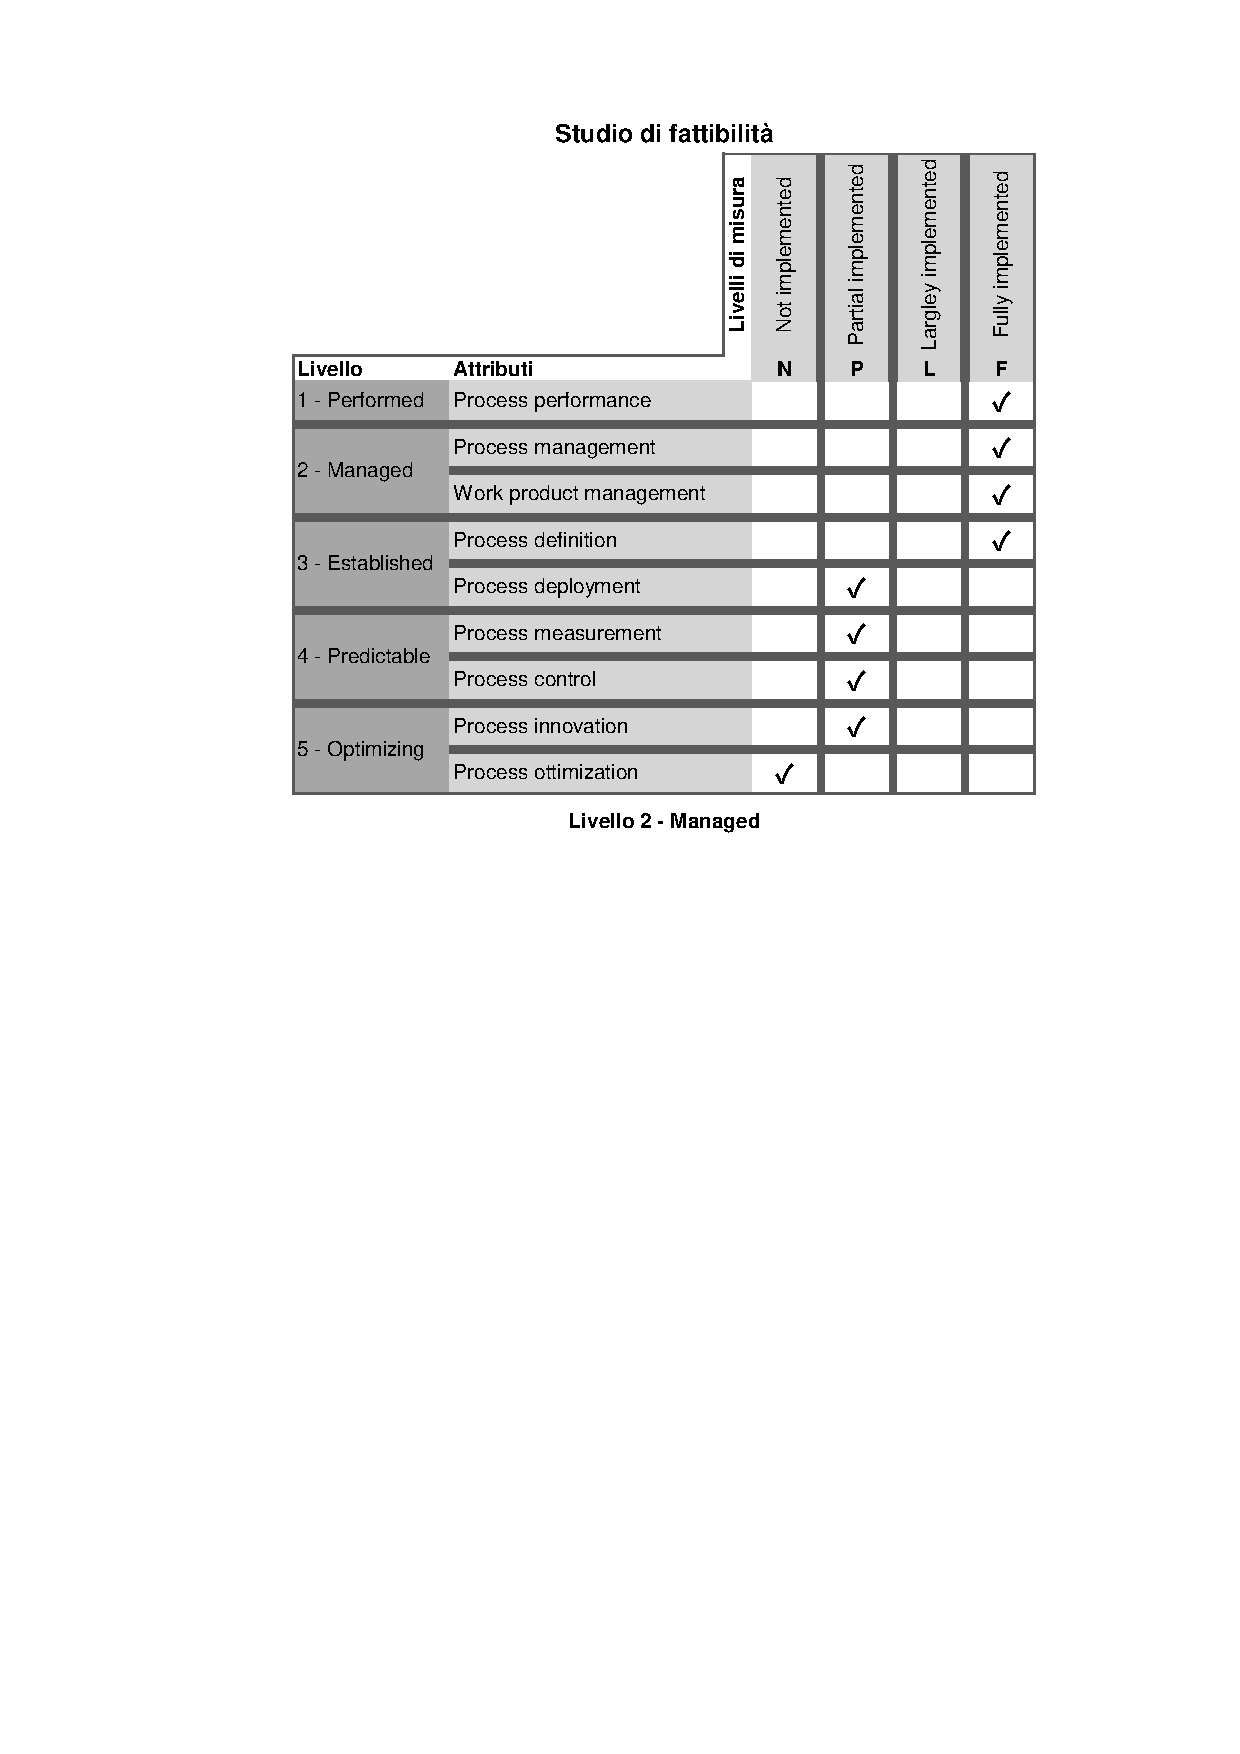
\includegraphics[scale=1]{images/resoconto/RR/studiodifattibilita-RR.pdf}
	\caption{Valori ISO/IEC 15504 Studio di fattibilità}	
\end{figure}
\newpage
\subparagraph{Norme di progetto}
\noindent
\begin{figure}[H]
	\centering
	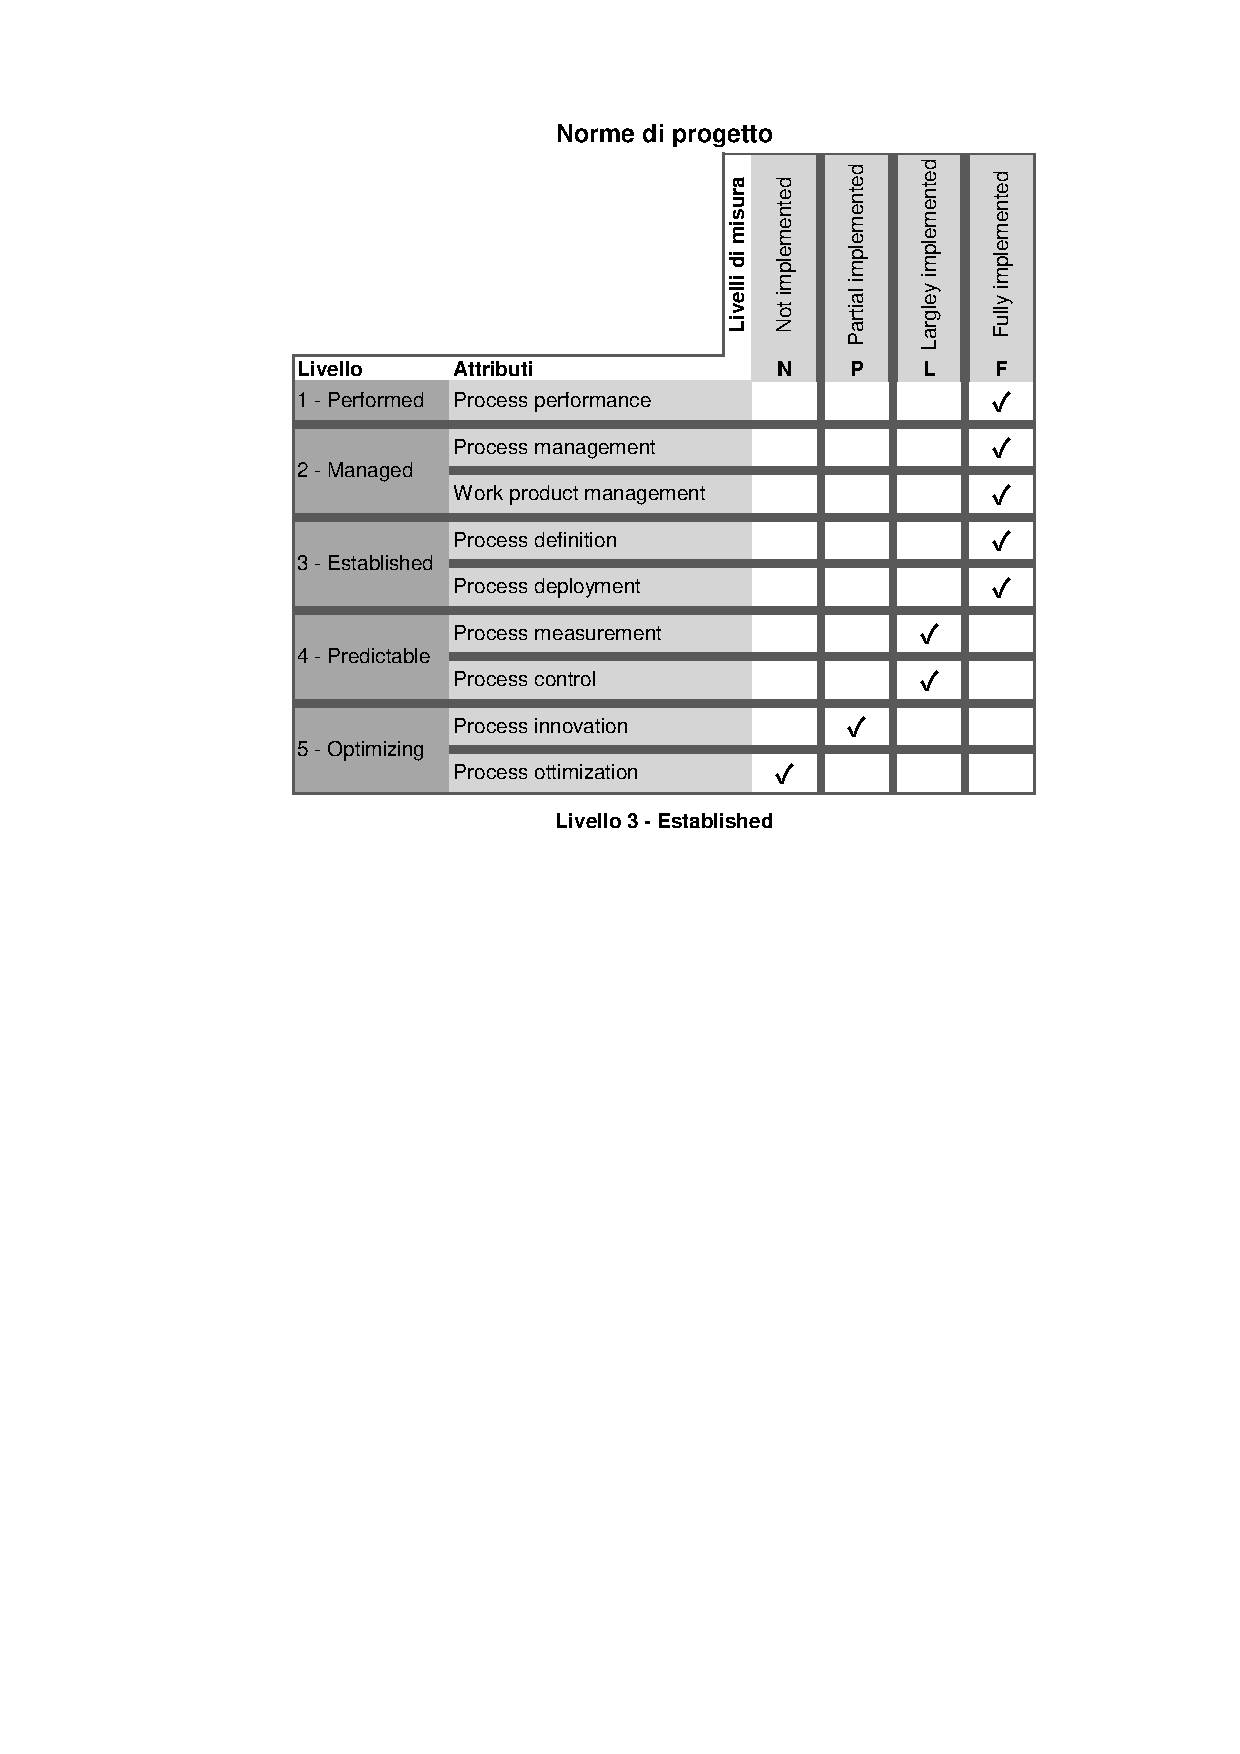
\includegraphics[scale=1]{images/resoconto/RR/normediprogetto-RR.pdf}
	\caption{Valori ISO/IEC 15504 Norme di progetto}	
\end{figure}
\newpage
\subparagraph{Analisi dei requisiti}
\noindent
\begin{figure}[H]
	\centering
	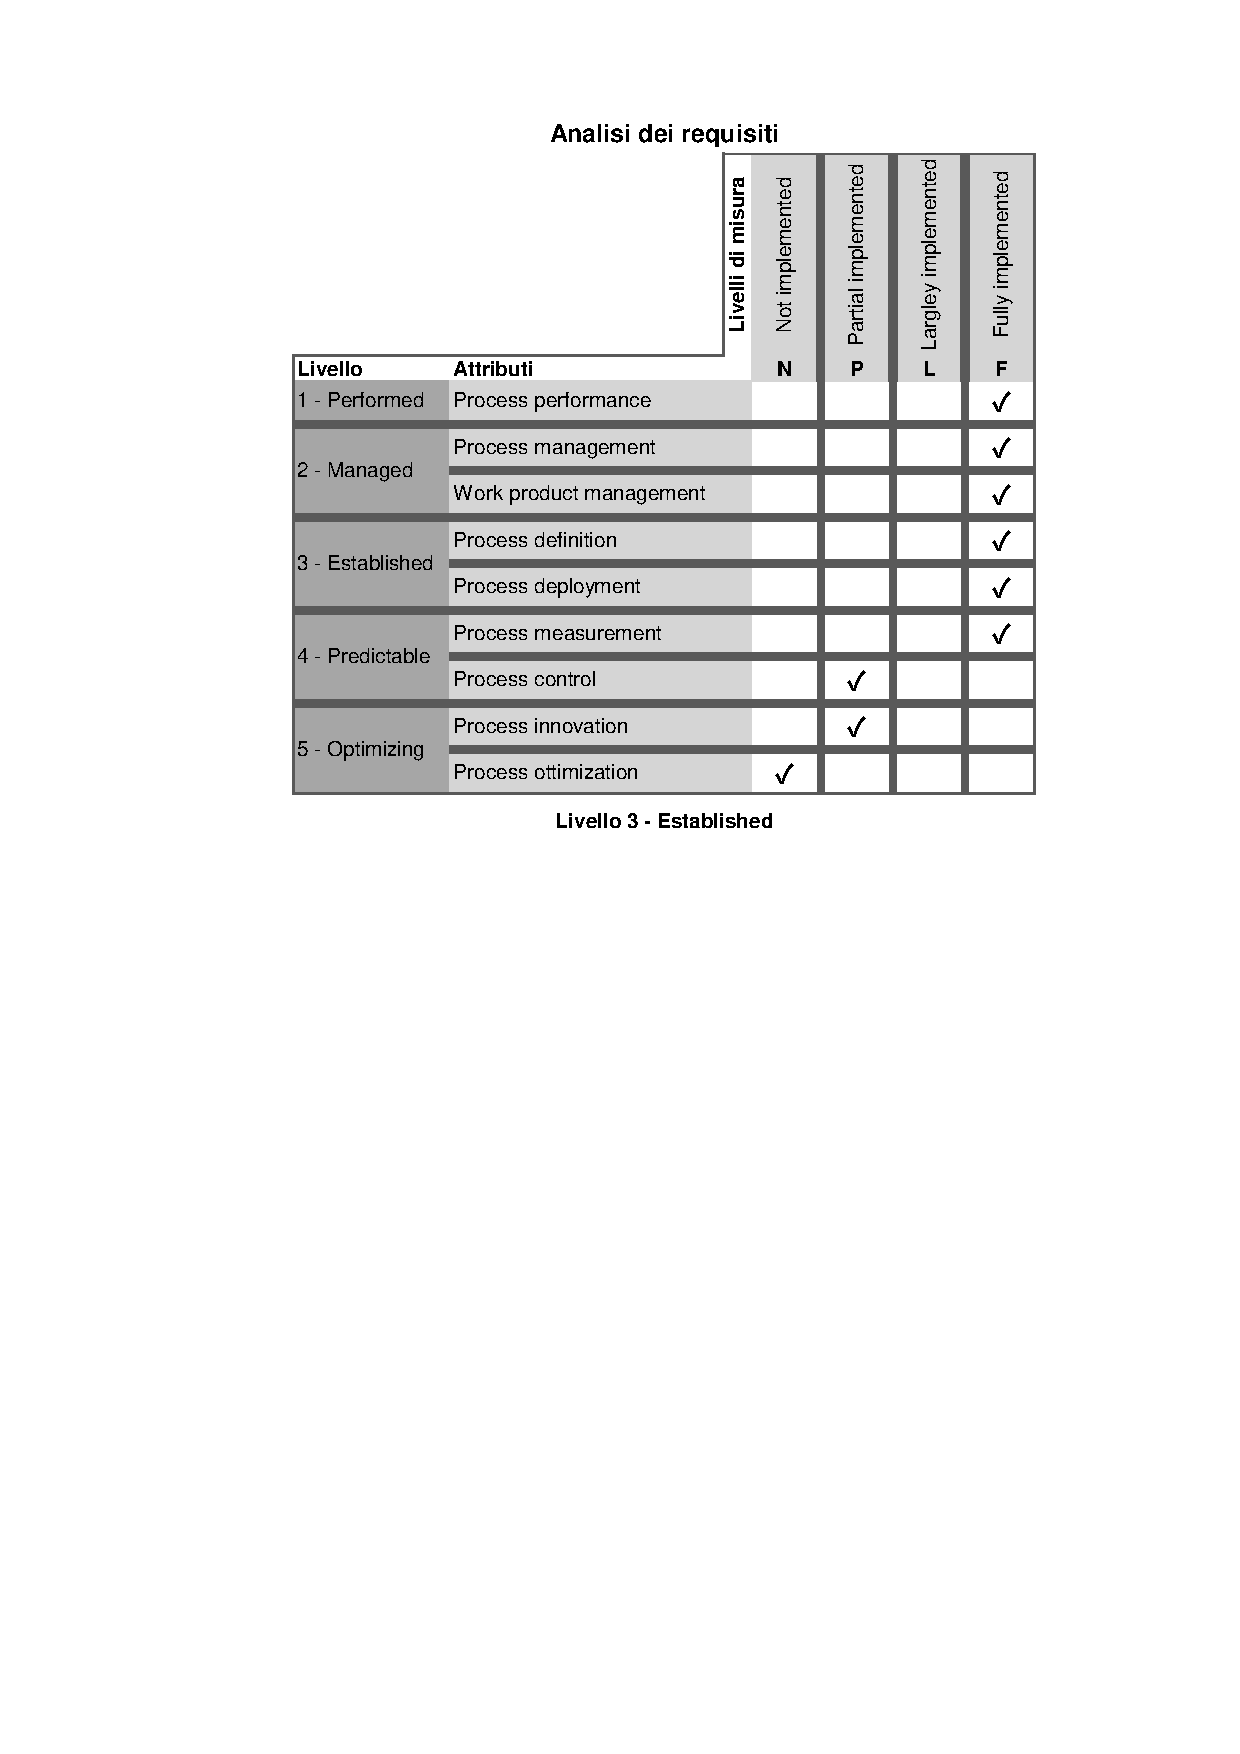
\includegraphics[scale=1]{images/resoconto/RR/analisideirequisiti-RR.pdf}
	\caption{Valori ISO/IEC 15504 Analisi dei requisiti}
\end{figure}
\newpage
\subparagraph{Pianificazione di progetto}
\noindent
\begin{figure}[H]
	\centering
	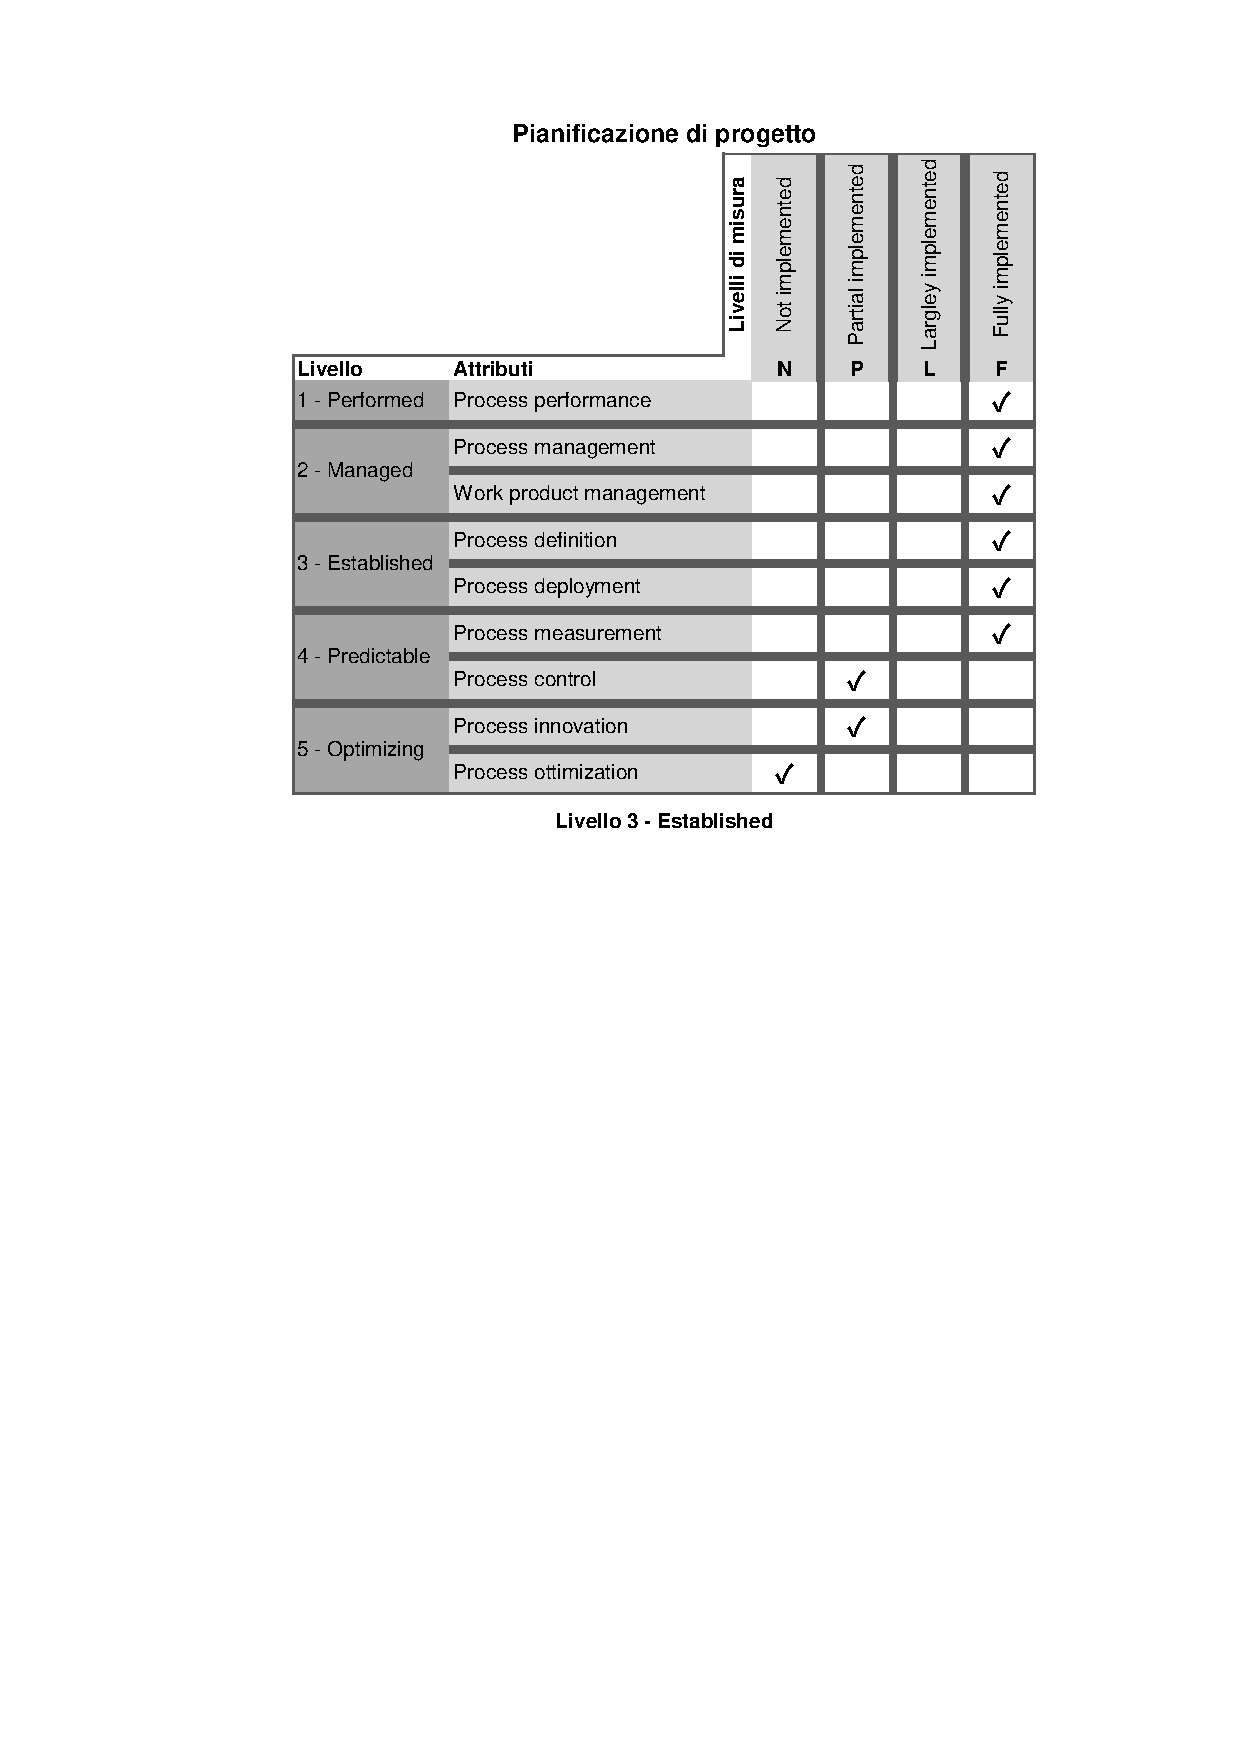
\includegraphics[scale=1]{images/resoconto/RR/pianificazioneprogetto-RR.pdf}
	\caption{Valori ISO/IEC 15504 Pianificazione di progetto}	
\end{figure}
\newpage
\subparagraph{Pianificazione di qualifica}
\noindent
\begin{figure}[H]
	\centering
	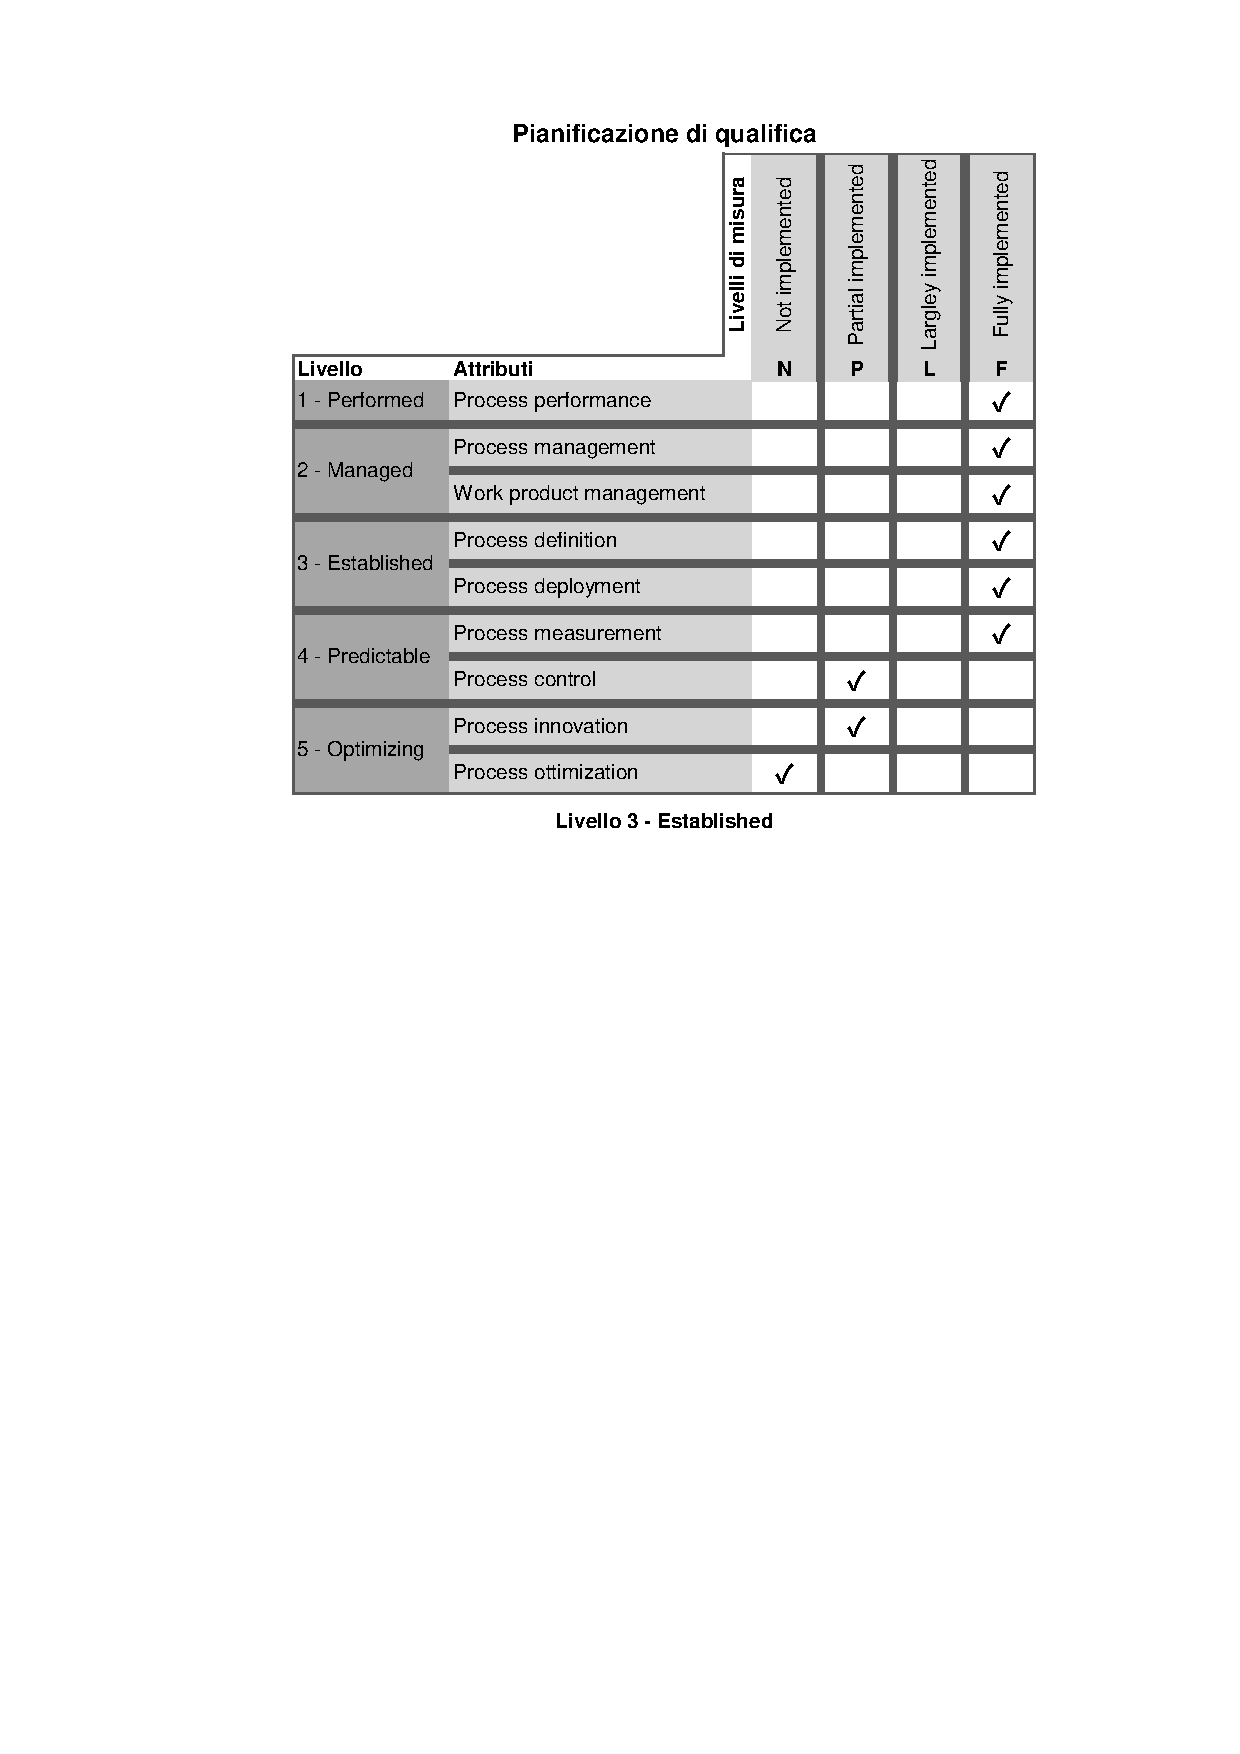
\includegraphics[scale=1]{images/resoconto/RR/pianificazionequalifica-RR.pdf}
	\caption{Valori ISO/IEC 15504 Pianificazione di qualifica}	
\end{figure}
\newpage

\subparagraph{Grafico riassuntivo}\noindent \\
Nel seguente grafico possiamo visualizzare una rappresentazione dei livelli raggiunti da ciascun processo implementato e quindi valutato durante il periodo della revisione dei requisiti. 

\begin{figure}[H]
	\centering
	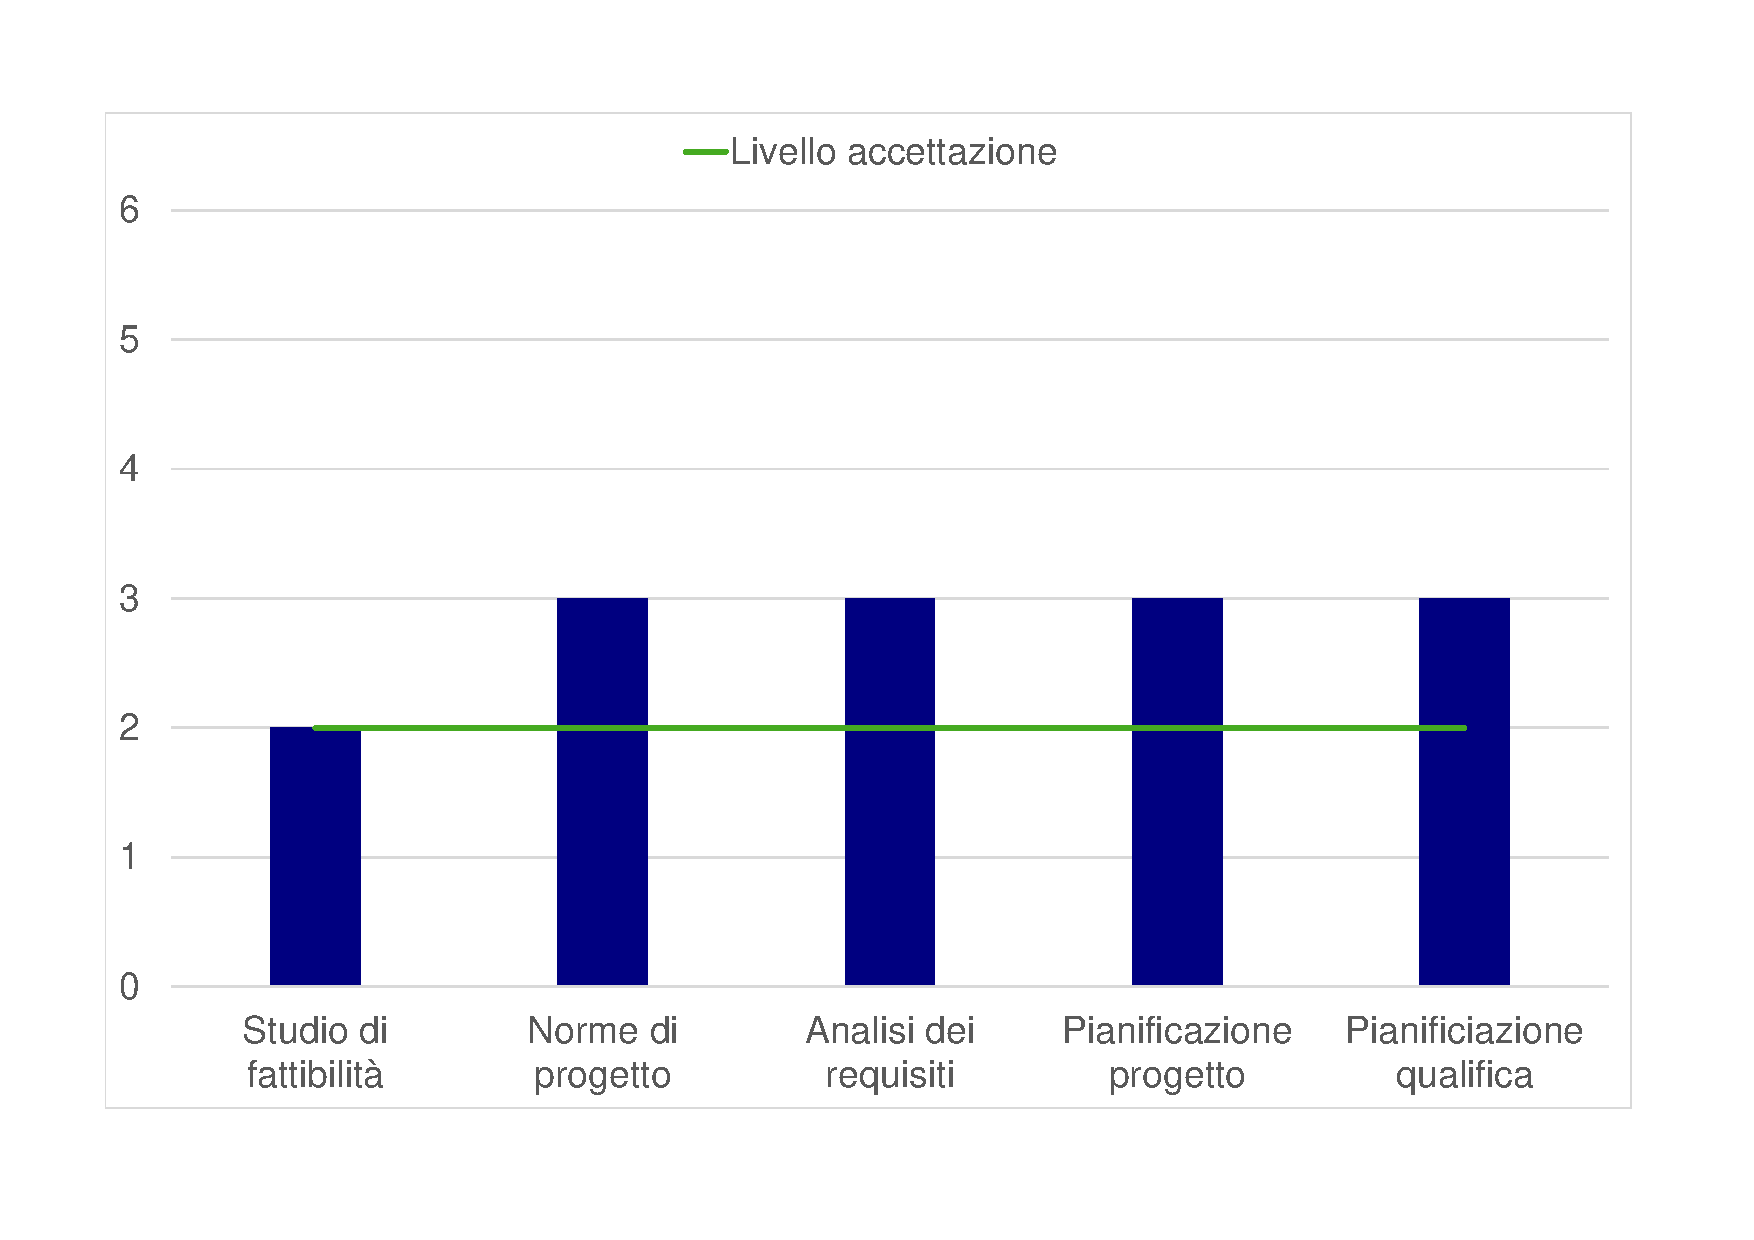
\includegraphics[scale=0.5]{images/resoconto/RR/chart-RR.pdf}
	\caption{Riassunto valori processi - Revisione dei requisiti}
\end{figure}

\newpage
\paragraph{Revisione di Progettazione \\}
Di seguito riportiamo le misurazioni dei processi più significativi sviluppati durante il periodo di Revisione di Progettazione. Tali valori sono stati raccolti secondo la metrica MPC1 che fa riferimento alle linee guida dettate dallo standard ISO/IEC 15504.
\subparagraph{Normazione}
\noindent
\begin{figure}[H]
	\centering
	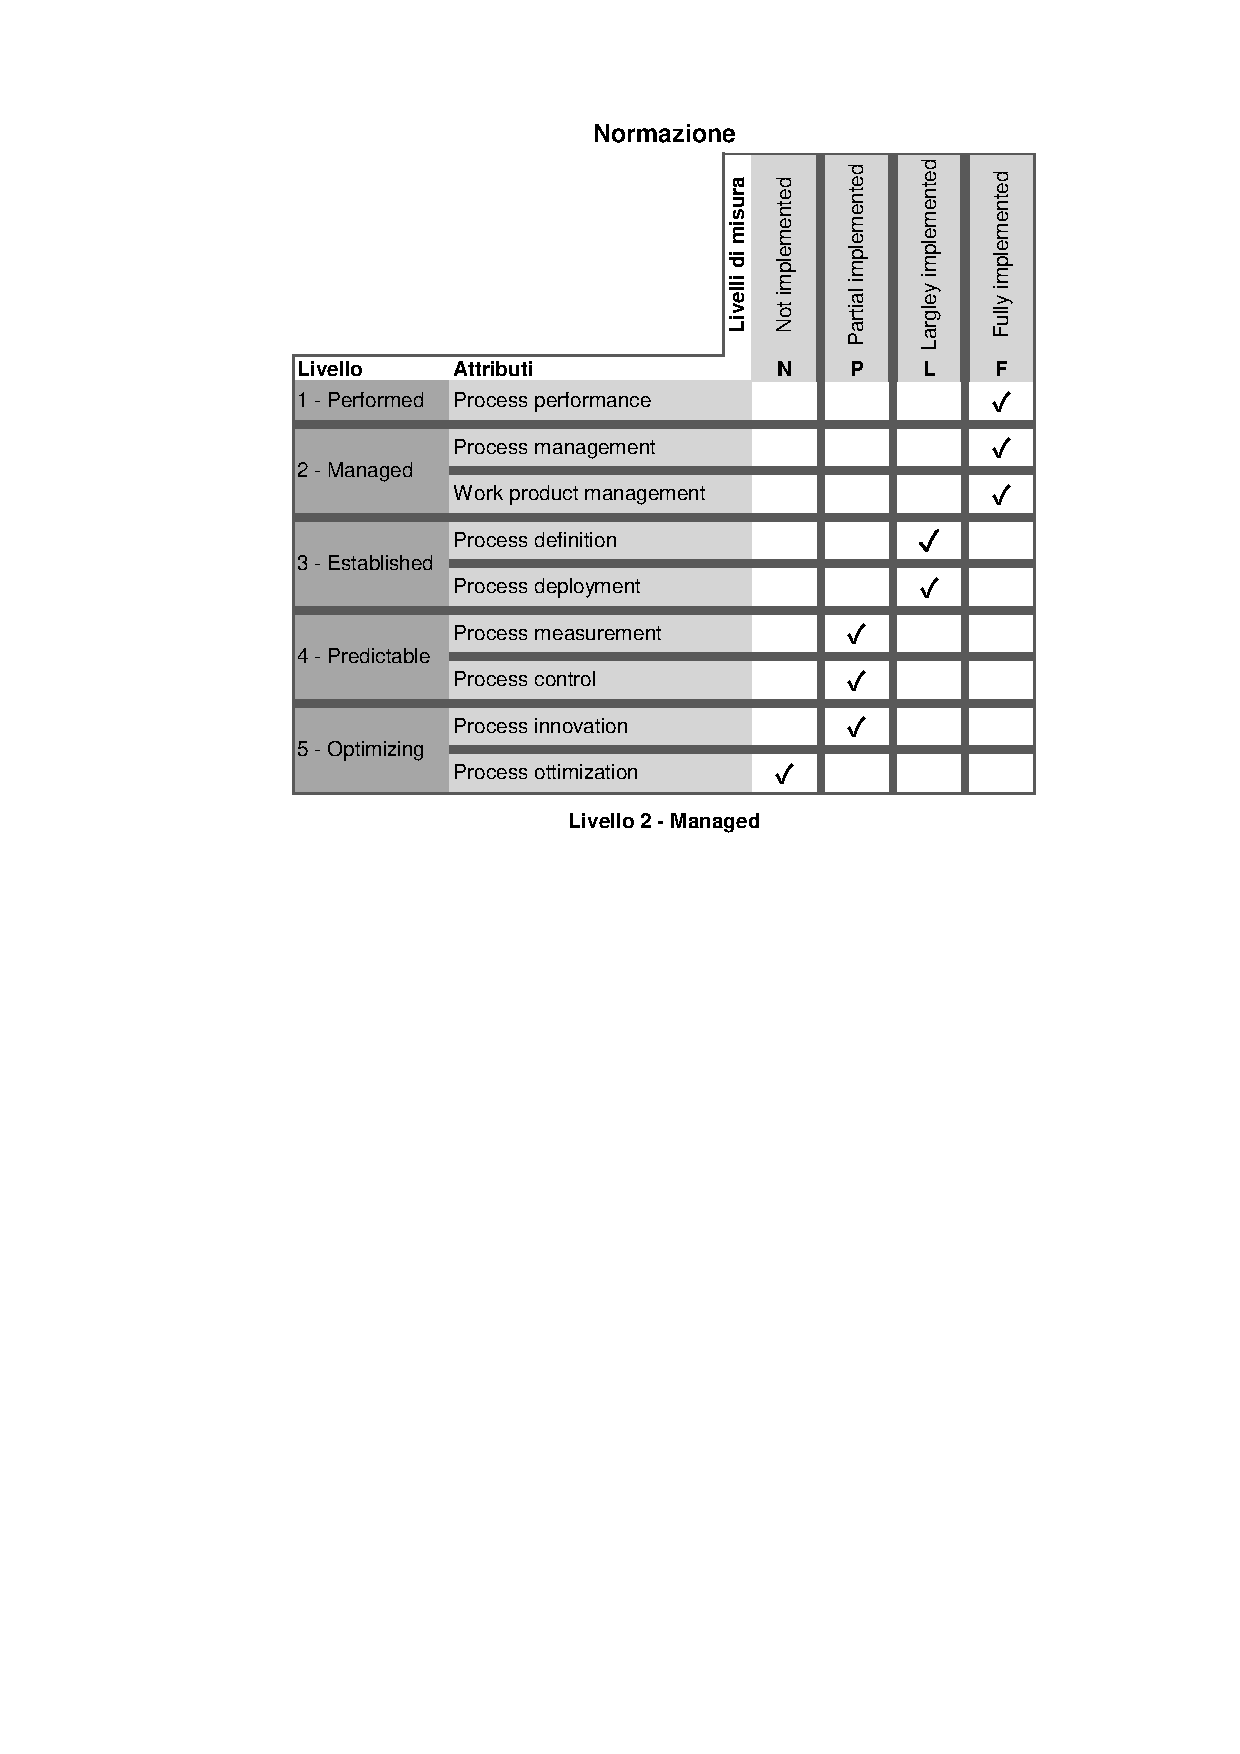
\includegraphics[scale=1]{images/resoconto/RP/normazione-RP.pdf}
	\caption{Valori ISO/IEC 15504 Pianificazione progetto}	
\end{figure}
\newpage
\subparagraph{Analisi dei requisiti}
\noindent
\begin{figure}[H]
	\centering
	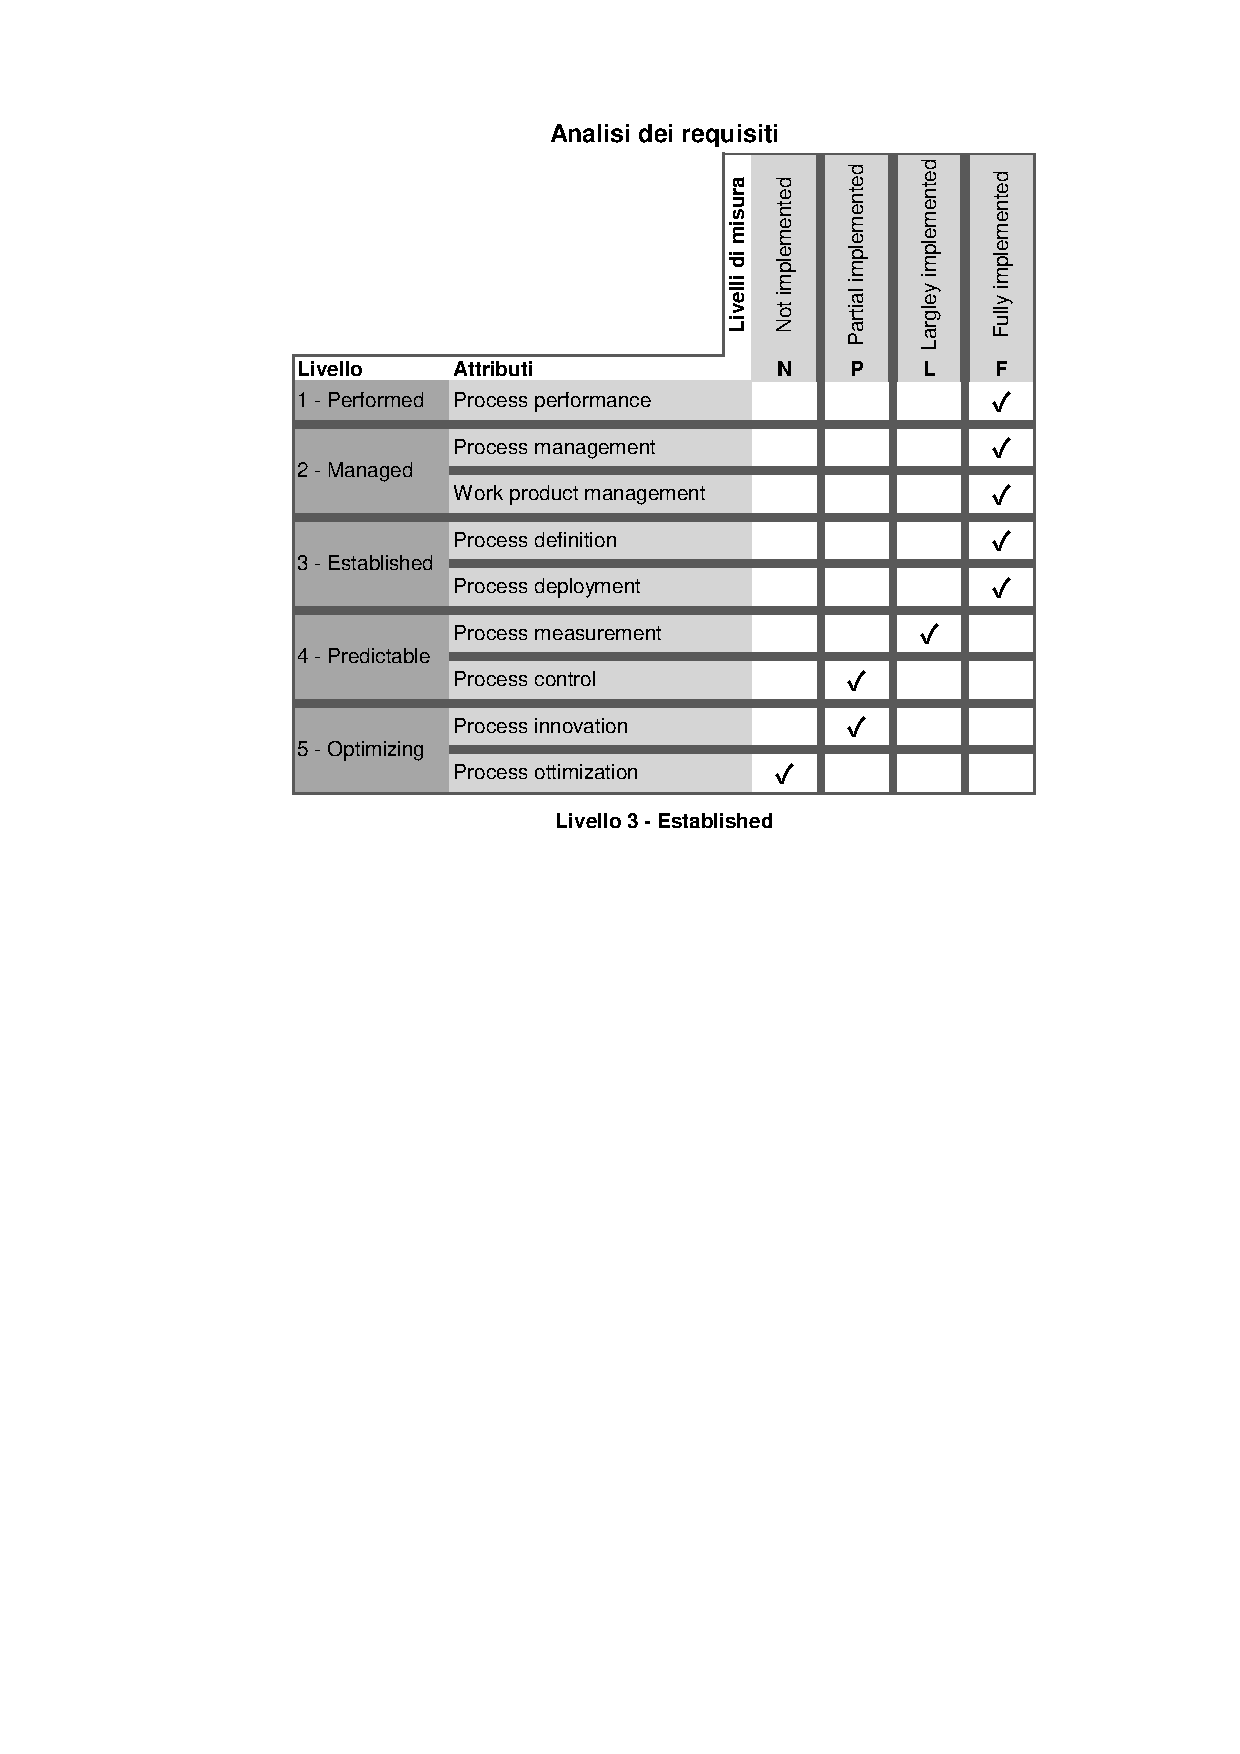
\includegraphics[scale=1]{images/resoconto/RP/analisideirequisiti-RP.pdf}
	\caption{Valori ISO/IEC 15504 Analisi dei requisiti}	
\end{figure}
\newpage
\subparagraph{Progettazione}
\noindent
\begin{figure}[H]
	\centering
	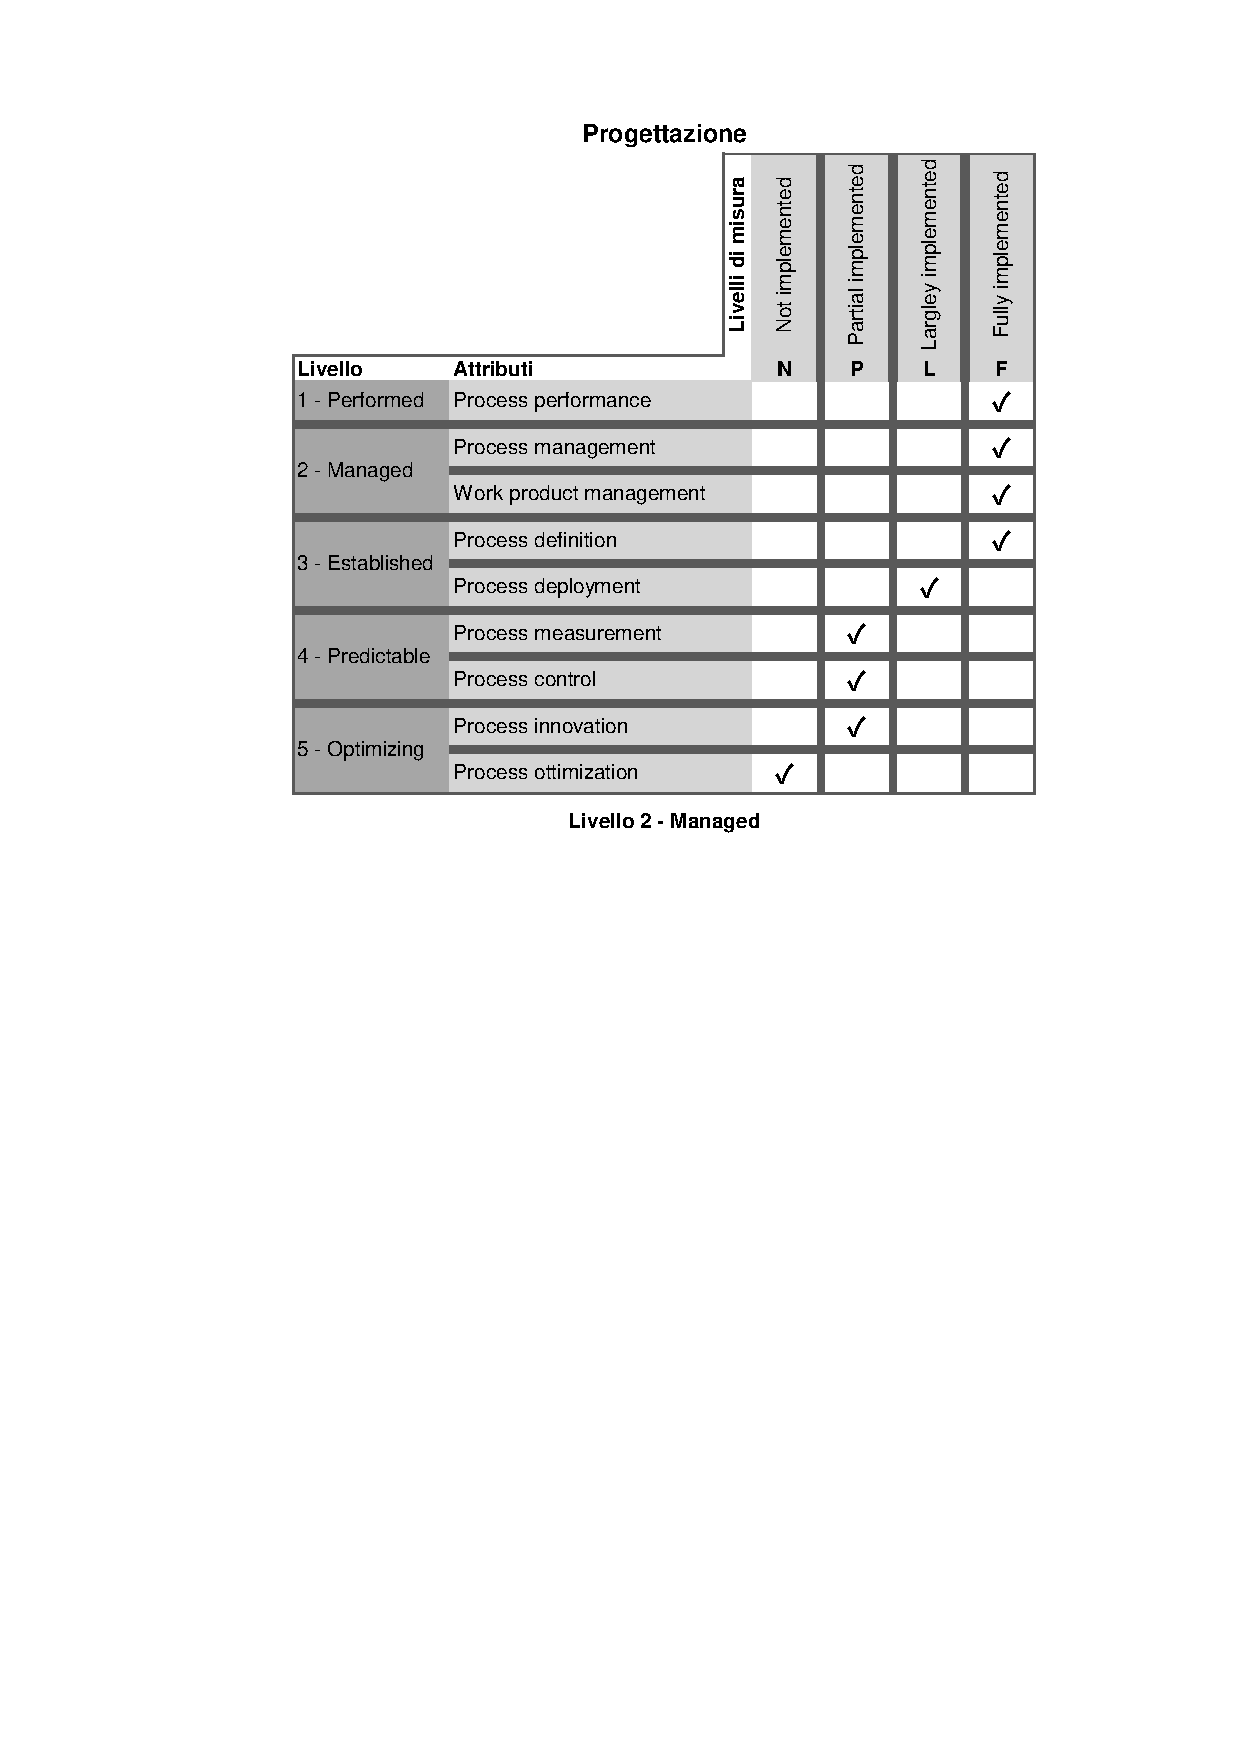
\includegraphics[scale=1]{images/resoconto/RP/progettazione-RP.pdf}
	\caption{Valori ISO/IEC 15504 Progettazione}	
\end{figure}
\newpage
\subparagraph{Documentazione}
\noindent
\begin{figure}[H]
	\centering
	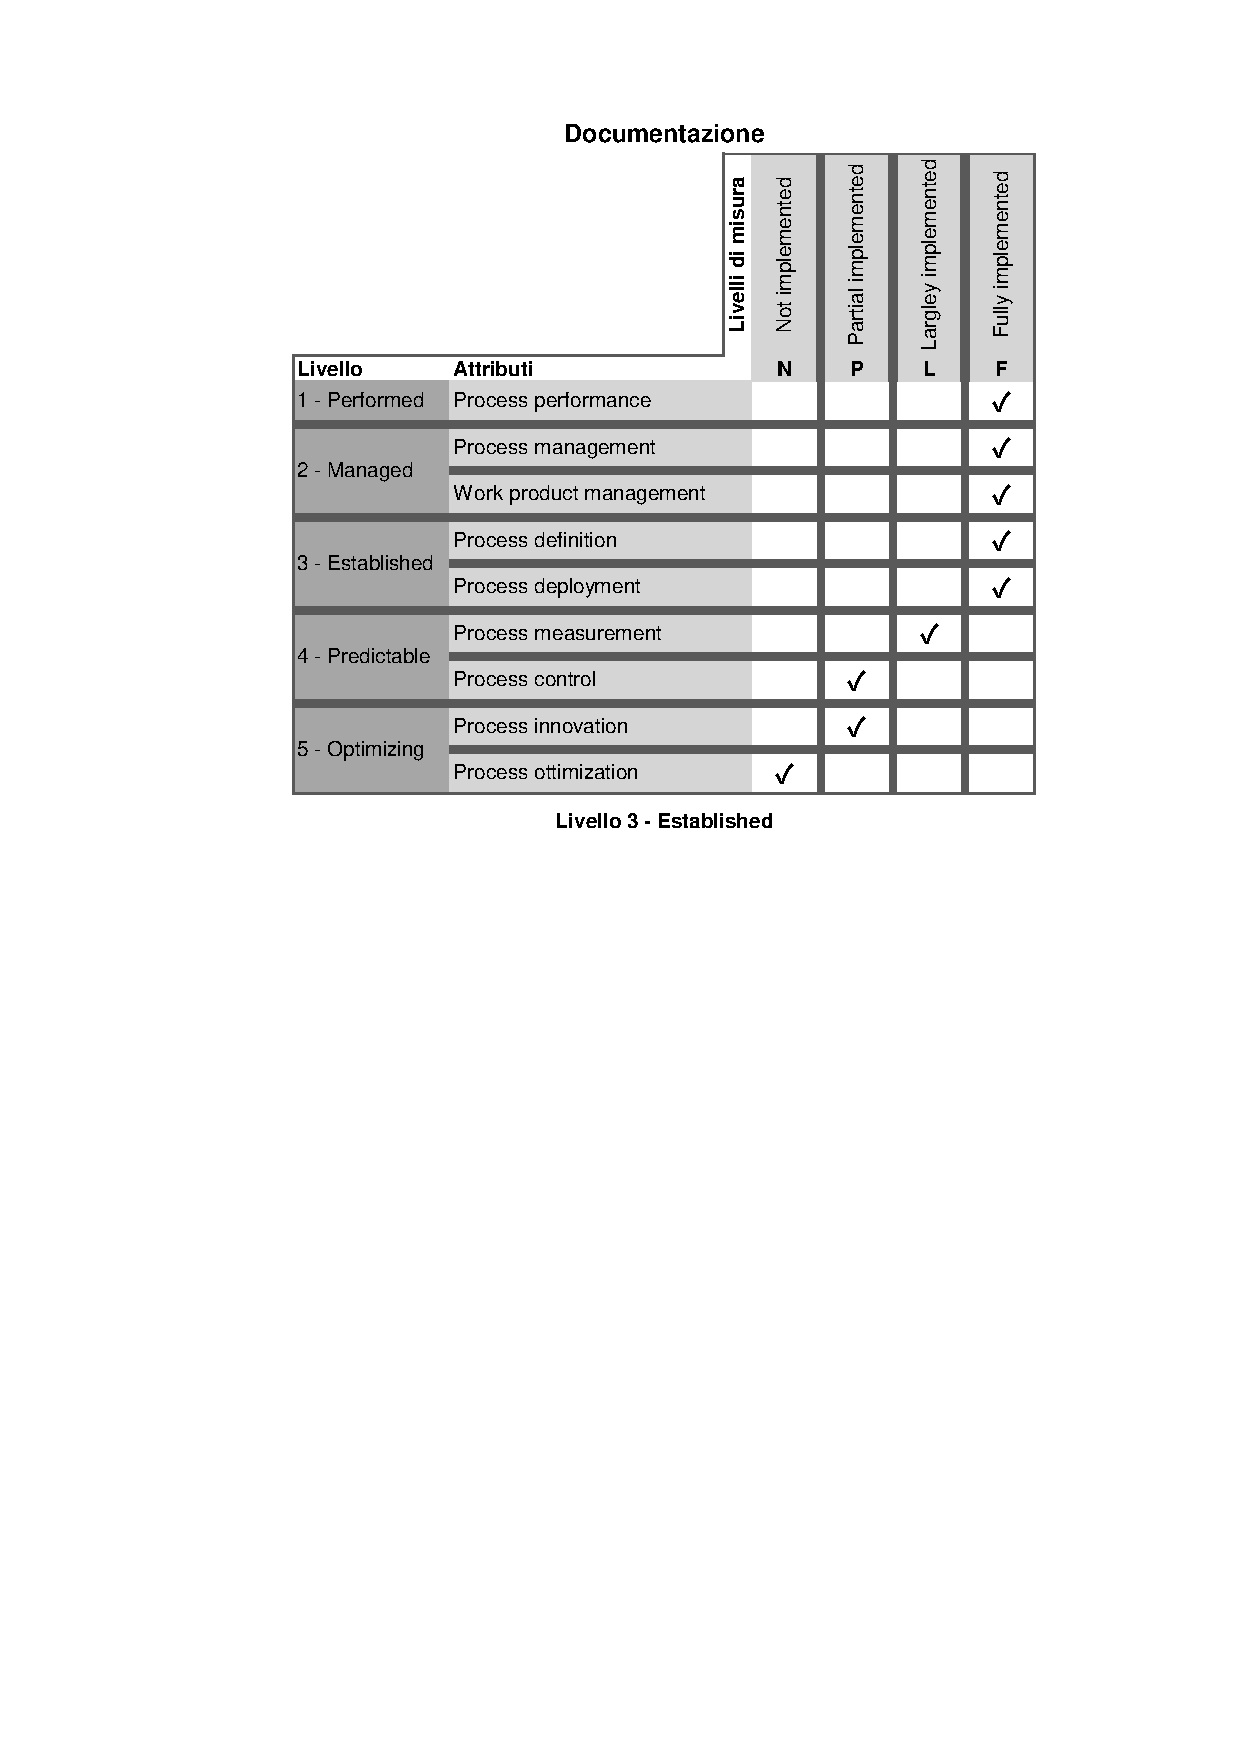
\includegraphics[scale=1]{images/resoconto/RP/documentazione-RP.pdf}
	\caption{Valori ISO/IEC 15504 Documentazione}	
\end{figure}
\newpage
\subparagraph{Pianificazione progetto}
\noindent
\begin{figure}[H]
	\centering
	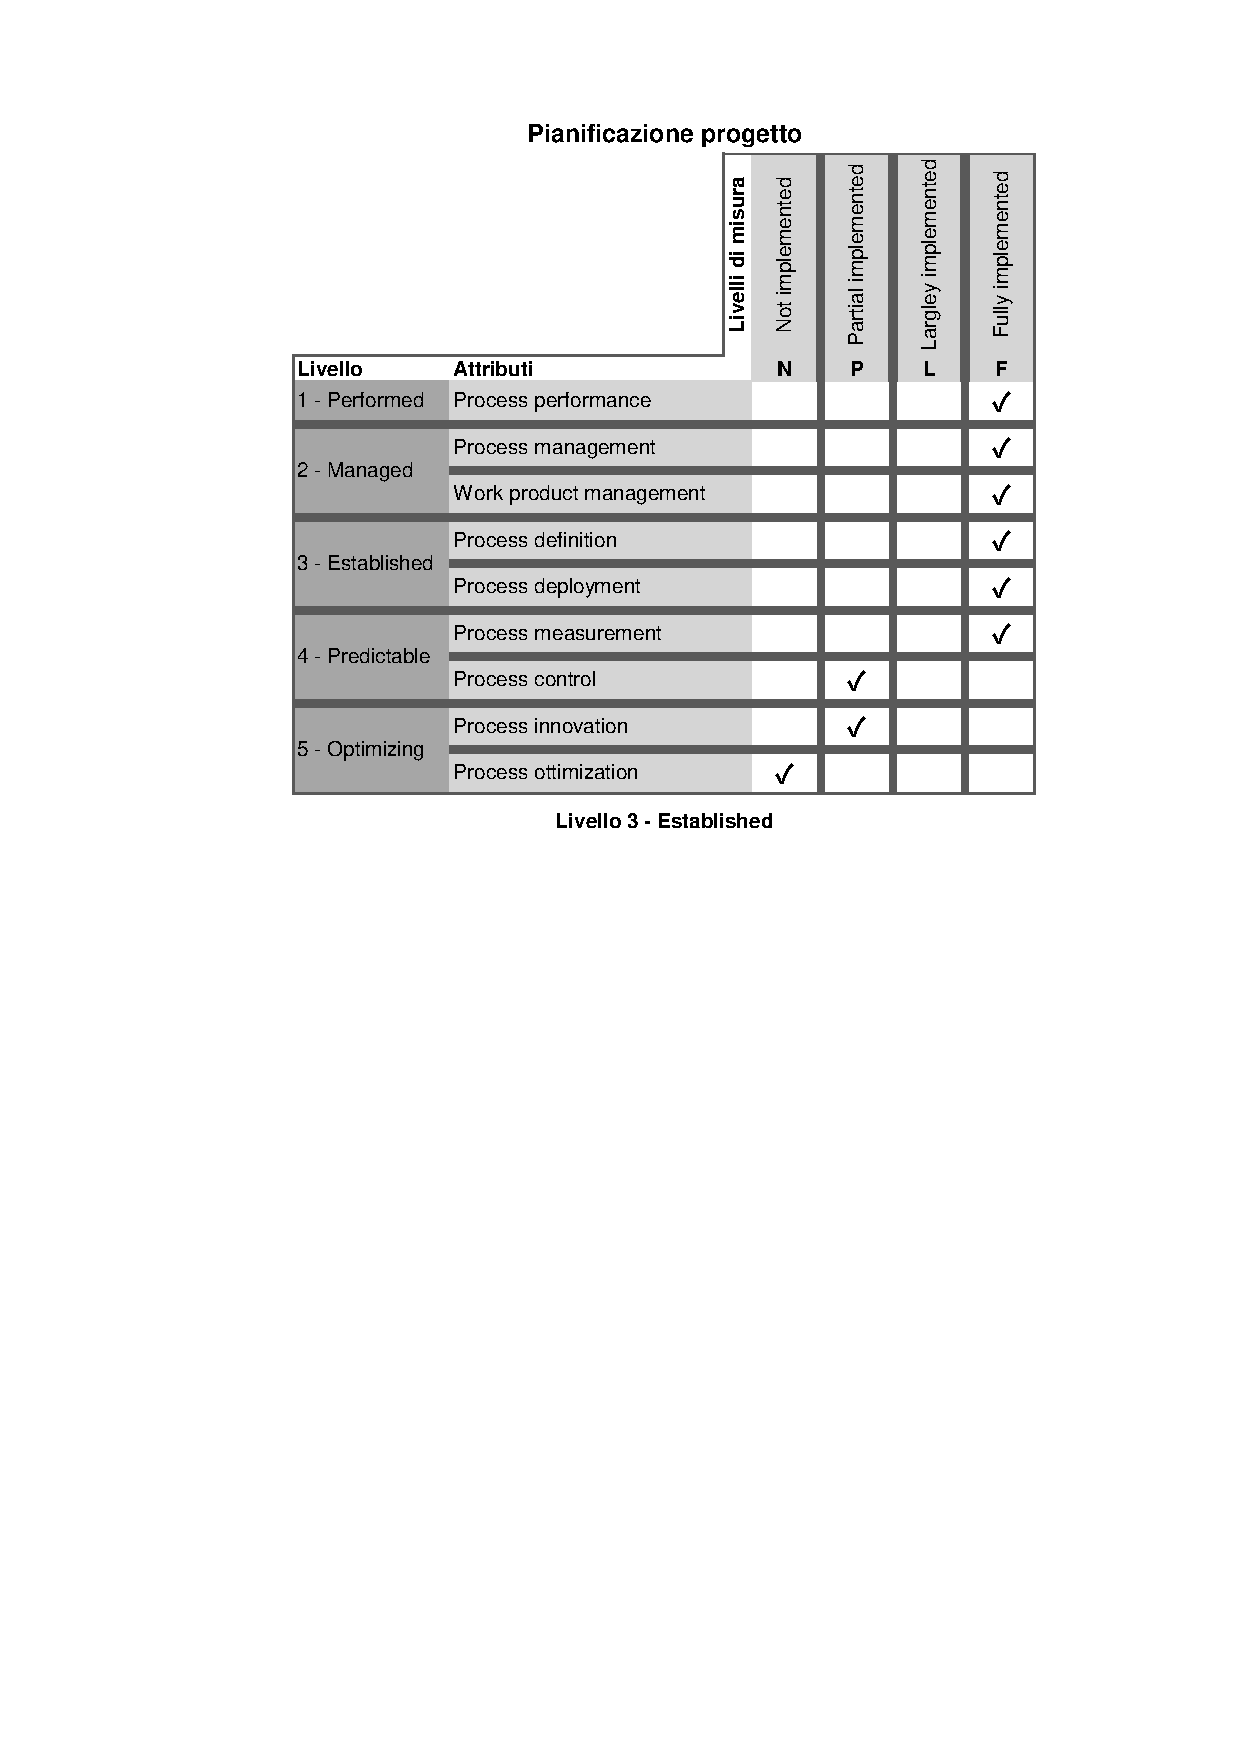
\includegraphics[scale=1]{images/resoconto/RP/pianificazioneprogetto-RP.pdf}
	\caption{Valori ISO/IEC 15504 Pianificazione progetto}	
\end{figure}
\newpage
\subparagraph{Ricerca delle tecnologie}
\noindent
\begin{figure}[H]
	\centering
	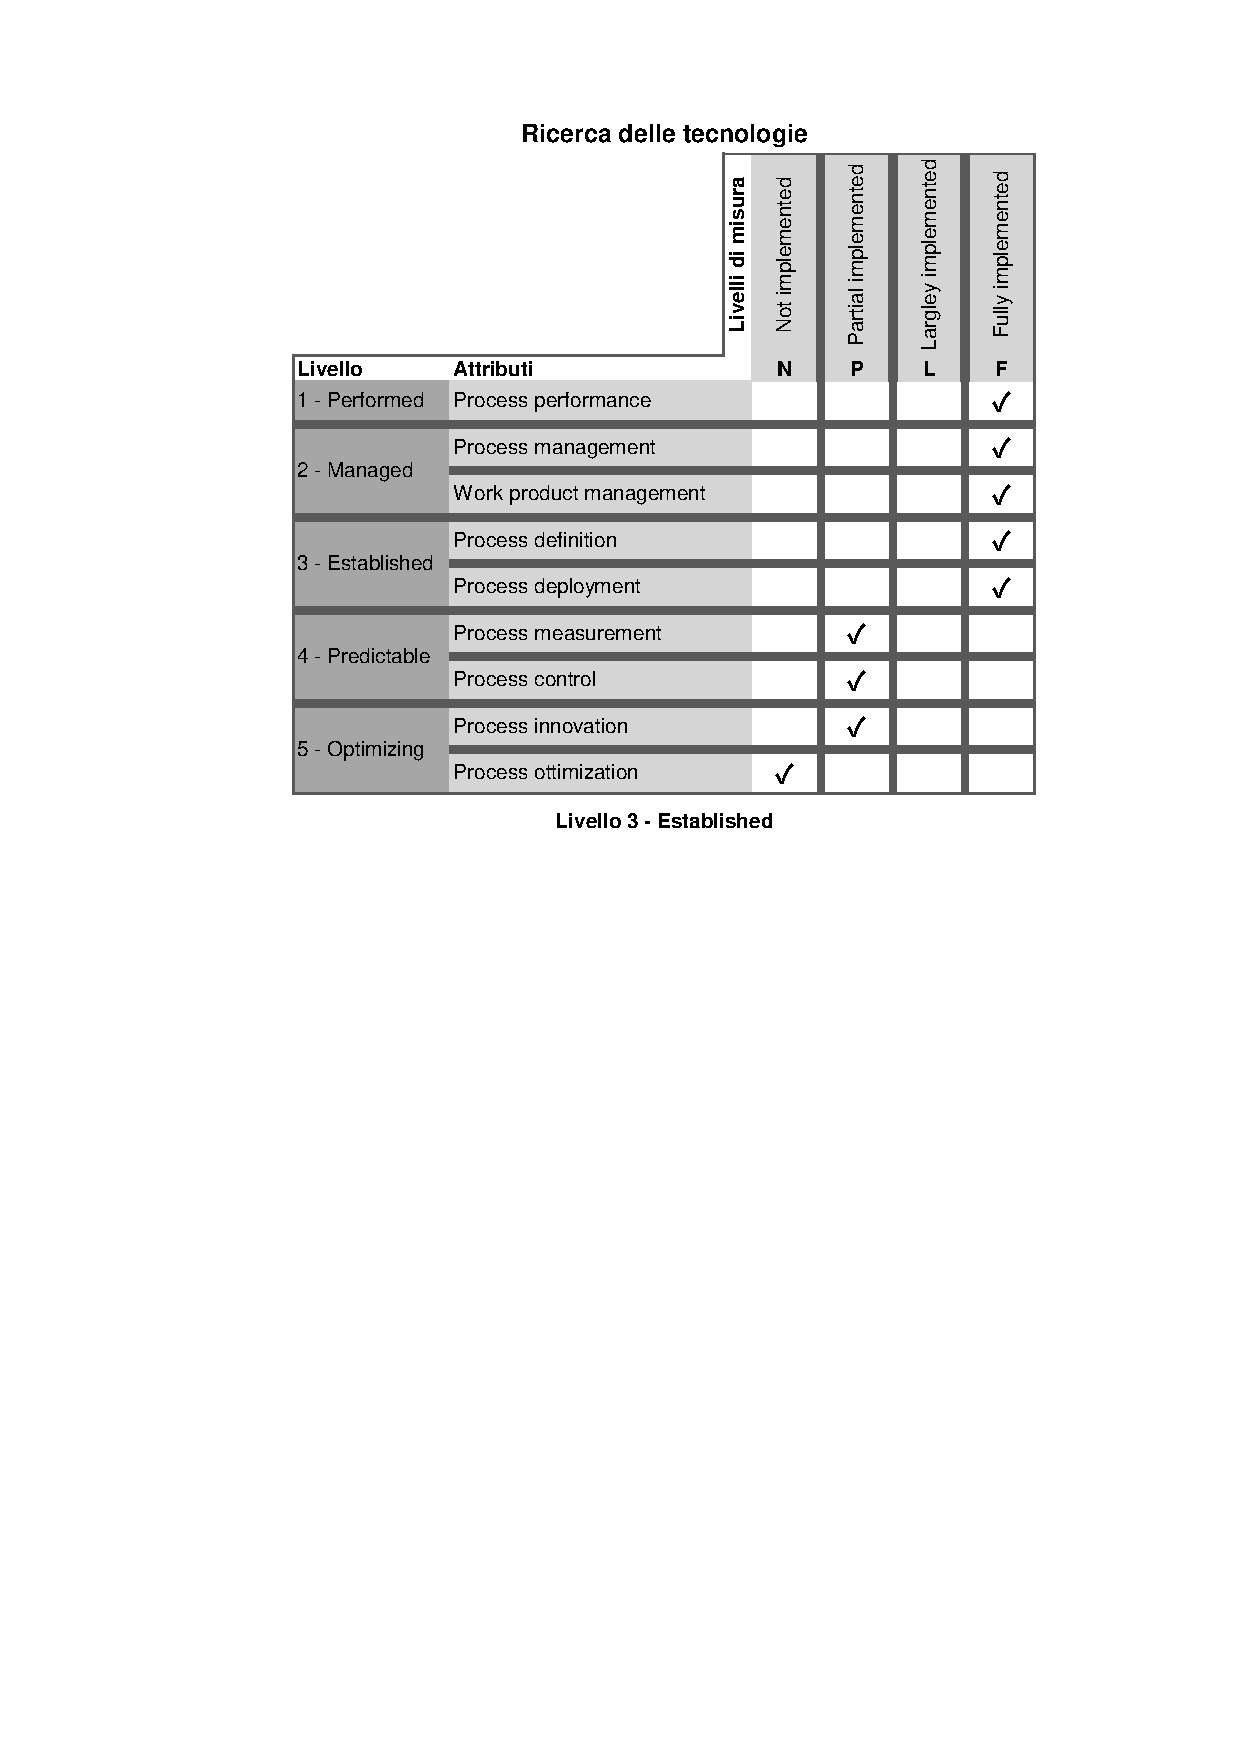
\includegraphics[scale=1]{images/resoconto/RP/ricercadelletecnologie-RP.pdf}
	\caption{Valori ISO/IEC 15504 Ricerca delle tecnologie}	
\end{figure}
\newpage

\subparagraph{Grafico riassuntivo}
\noindent \\
Nel seguente grafico possiamo visualizzare una rappresentazione dei livelli raggiunti da ciascun processo implementato e quindi valutato durante il periodo della revisione di progetto. 

\begin{figure}[H]
	\centering
	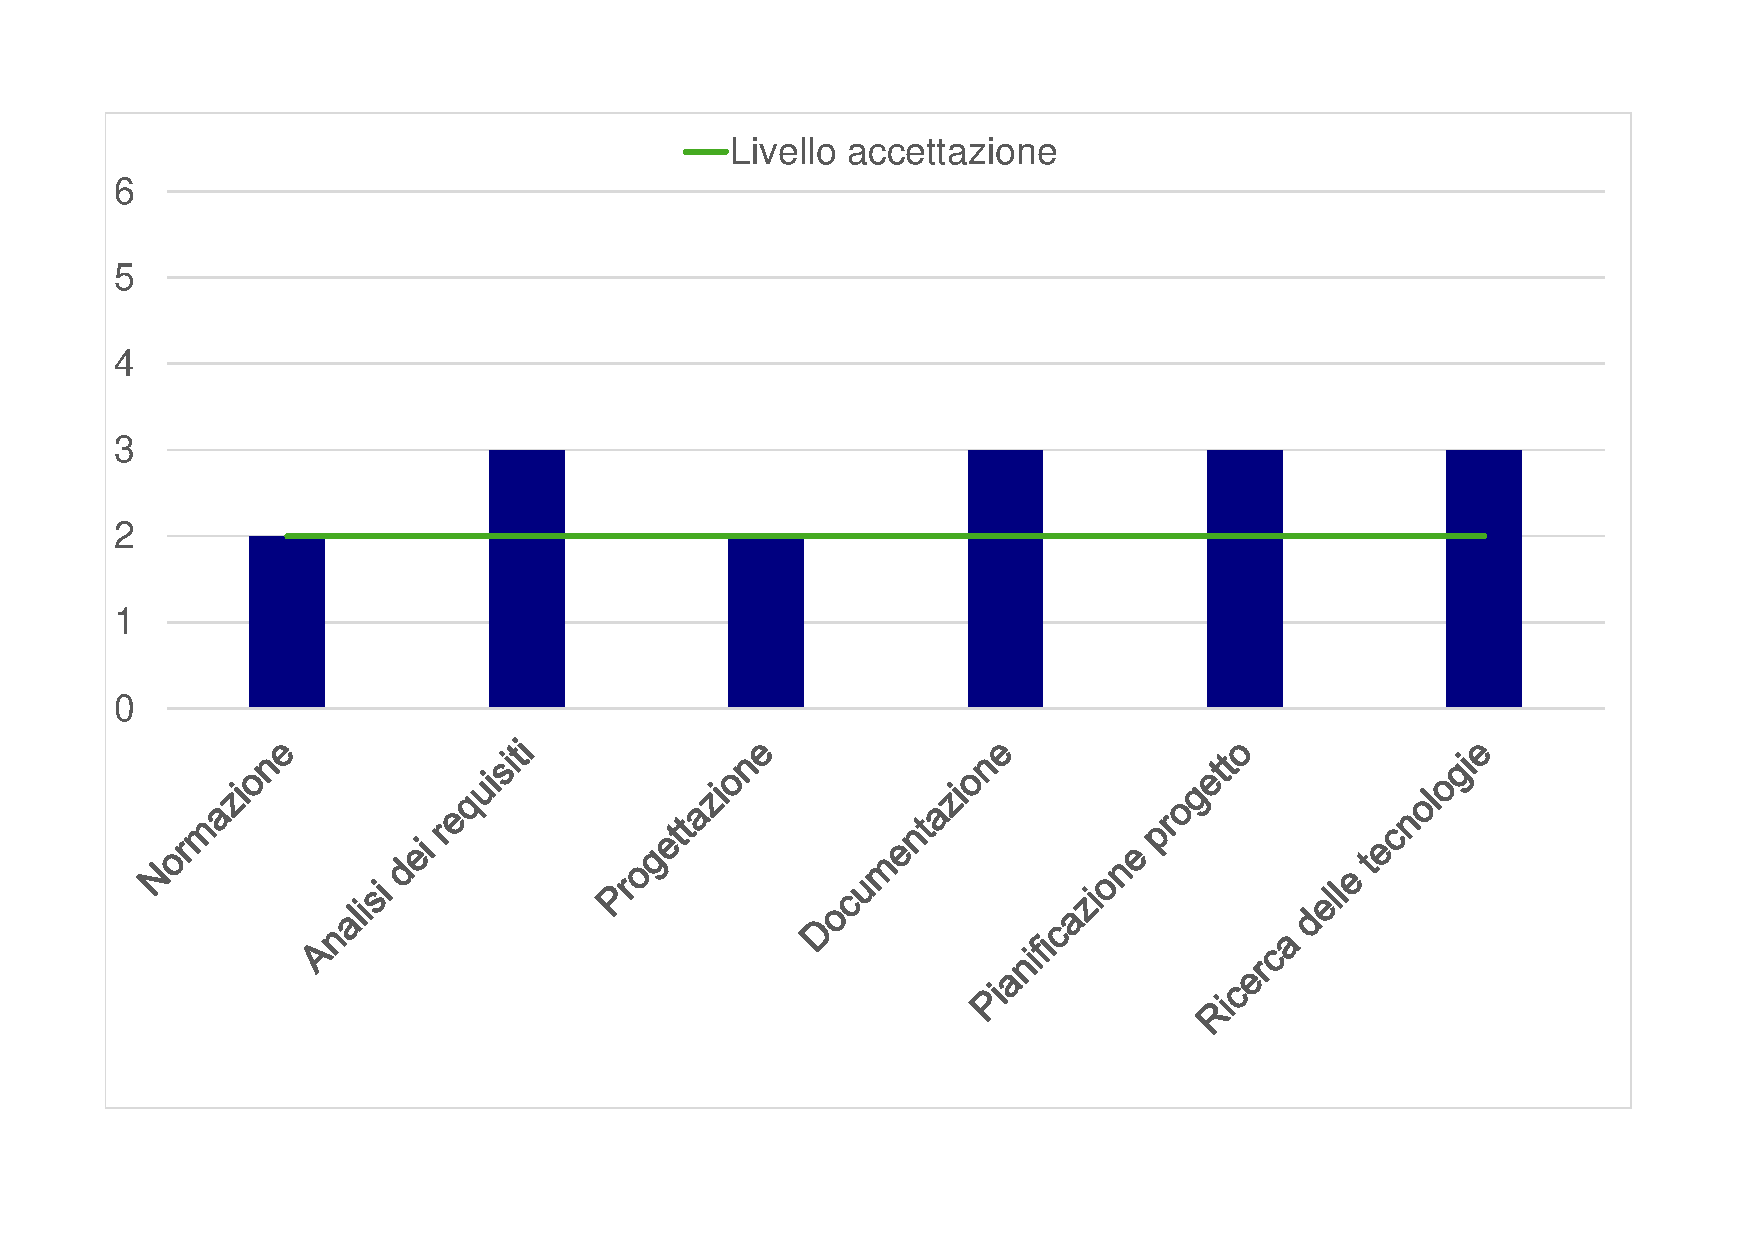
\includegraphics[scale=0.5]{images/resoconto/RP/chart-RP.pdf}
	\caption{Riassunto valori processi - Revisione di progetto}	
\end{figure}
\newpage
\subsection{Requisiti}
\subsubsection{Valori Requirement Stability Index - MPC2}
\paragraph{Revisione di progetto\\}
Durante il periodo di Revisione di progetto abbiamo individuato periodicamente tutti i cambiamenti apportati ai requisiti del progetto. Questo ci ha permesso di determinare la stabilità dei requisiti nel tempo grazie all'utilizzo della metrica MPC2.
Riportiamo di seguito i calcoli e le varie rilevazioni effettuate.

\begin{longtable}{>{\centering\arraybackslash}m{3cm} >{\centering\arraybackslash}m{4cm} >{\centering\arraybackslash}m{5cm} >{\centering\arraybackslash}m{2cm}}
	\rowcolor{LightBlue}
	\textbf{\textcolor{white}{Data rilevazioni}}
	& \textbf{\textcolor{white}{Requirement Stability Index (RSI)}}
	& \textbf{\textcolor{white}{Esito}}\\
	
	2019-02-15 & \[1-\frac{0+5+4}{48}=0.81\] & Accettato\\
	\hline
	2019-02-20 & \[1-\frac{5+0+3}{43}=0.81\] & Accettato\\
	\hline
	2019-02-21 & \[1-\frac{8+0+3}{48}=0.77\] & Accettato\\
	\hline
	2019-02-22 & \[1-\frac{5+2+0}{56}=0.85\] & Accettato\\
	\hline
	2019-02-25 & \[1-\frac{11+0+0}{59}=0.81\] & Accettato\\
	\hline
	2019-02-27 & \[1-\frac{8+0+0}{70}=0.88\] & Accettato\\
	\hline
	2019-03-04 & \[1-\frac{11+0+0}{78}=0.86\] & Accettato\\
	\hline
	2019-03-05 & \[1-\frac{14+0+1}{89}=0.83\] & Accettato\\
	\hline\\
	\caption{Rilevazioni indice stabilità requisiti (RSI) - Revisione di progetto}
\end{longtable}
\begin{figure}[H]
	\centering
	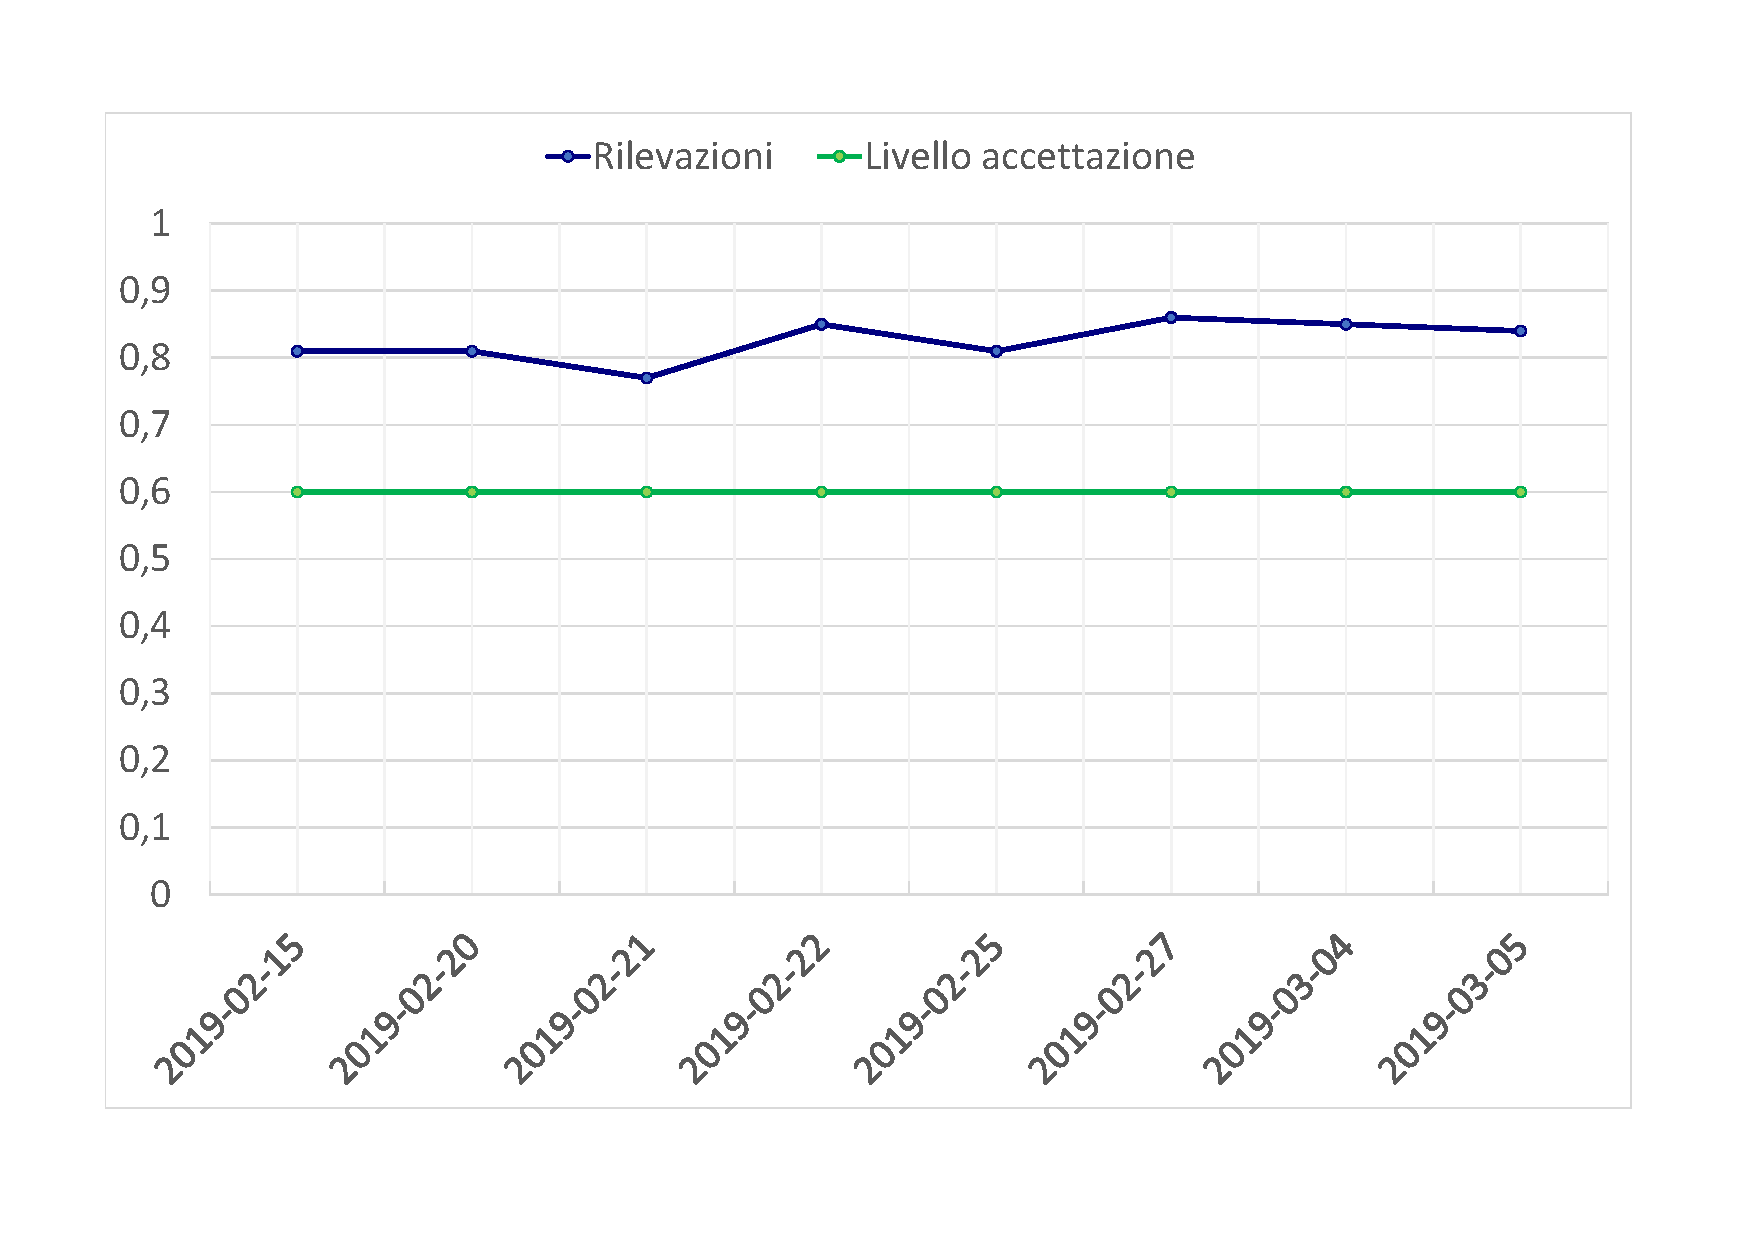
\includegraphics[scale=0.5]{images/resoconto/requisitiChart.pdf}
	\caption{Serie storica rilevazioni stabilità requisiti - Revisione di progetto}	
\end{figure}

\section{Copertura dei requisiti}
Viene riportata in seguito una tabella riassuntiva dei requisiti che non è da considerarsi definitiva, verrà infatti aggiornata in seguito ad ogni avanzamento significativo. \\
I requisiti sono indicati con il loro codice identificativo definito nel documento \textit{NormeDiProgetto\_v2.0.0} e la loro descrizione dettagliata è riportata nel documento \textit{AnalisiDeiRequisiti\_v2.0.0}.
\begin{longtable}{| p{2.5cm} | p{3cm} |}
	\rowcolor{LightBlue}
	\color{white}\bfseries Requisito & \color{white}\bfseries Stato \\
	ROF1 & Non soddisfatto \\ \hline
	ROF2 & Non soddisfatto \\ \hline
	ROF3 & Non soddisfatto \\ \hline
	ROF4 & Non soddisfatto \\ \hline
	ROF5 & Non soddisfatto \\ \hline
	ROF6 & Non soddisfatto \\ \hline
	ROF7 & Non soddisfatto \\ \hline
	ROF8 & Non soddisfatto \\ \hline
	ROF9 & Non soddisfatto \\ \hline
	ROF10 & Non soddisfatto \\ \hline
	ROF11 & Non soddisfatto \\ \hline
	ROF12 & Non soddisfatto \\ \hline
	ROF13 & Non soddisfatto \\ \hline
	ROF14 & Non soddisfatto \\ \hline
	ROF15 & Non soddisfatto \\ \hline
	ROF16 & Non soddisfatto \\ \hline
	ROF17 & Non soddisfatto \\ \hline
	ROF18 & Non soddisfatto \\ \hline
	ROF19 & Non soddisfatto \\ \hline
	ROF20 & Non soddisfatto \\ \hline
	ROF21 & Non soddisfatto \\ \hline
	ROF22 & Non soddisfatto \\ \hline
	ROF23 & Non soddisfatto \\ \hline
	RDF1 & Non soddisfatto \\ \hline
	RDF2 & Non soddisfatto \\ \hline
	RDF3 & Non soddisfatto \\ \hline
	RDF4 & Non soddisfatto \\ \hline
	RDF5 & Non soddisfatto \\ \hline
	RDF6 & Non soddisfatto \\ \hline
	RDF7 & Non soddisfatto \\ \hline
	RDF8 & Non soddisfatto \\ \hline
	RDF9 & Non soddisfatto \\ \hline
	RDF10 & Non soddisfatto \\ \hline
	RDF11 & Non soddisfatto \\ \hline
	RDF12 & Non soddisfatto \\ \hline
	RDF13 & Non soddisfatto \\ \hline
	RDF14 & Non soddisfatto \\ \hline
	RDF15 & Non soddisfatto \\ \hline
	RDF16 & Non soddisfatto \\ \hline
	RDF17 & Non soddisfatto \\ \hline
	RDF18 & Non soddisfatto \\ \hline
	RDF19 & Non soddisfatto \\ \hline
	RDF20 & Non soddisfatto \\ \hline
	RDF21 & Non soddisfatto \\ \hline
	RDF22 & Non soddisfatto \\ \hline
	RDF23 & Non soddisfatto \\ \hline
	RDF24 & Non soddisfatto \\ \hline
	RDF25 & Non soddisfatto \\ \hline
	RPF1 & Non soddisfatto \\ \hline
	RPF2 & Non soddisfatto \\ \hline
	RPF3 & Non soddisfatto \\ \hline
	RPF4 & Non soddisfatto \\ \hline
	RPF5 & Non soddisfatto \\ \hline
	RPF6 & Non soddisfatto \\ \hline
	RPF7 & Non soddisfatto \\ \hline
	RPF8 & Non soddisfatto \\ \hline
	RPF9 & Non soddisfatto \\ \hline
	RPF10 & Non soddisfatto \\ \hline
	RPF11 & Non soddisfatto \\ \hline
	RPF12 & Non soddisfatto \\ \hline
	RPF13 & Non soddisfatto \\ \hline
	RPF14 & Non soddisfatto \\ \hline
	RPF15 & Non soddisfatto \\ \hline
	RPF16 & Non soddisfatto \\ \hline
	RPF17 & Non soddisfatto \\ \hline
	RPF18 & Non soddisfatto \\ \hline
	RPF19 & Non soddisfatto \\ \hline
	RPF20 & Non soddisfatto \\ \hline
	RPF21 & Non soddisfatto \\ \hline
	RPF22 & Non soddisfatto \\ \hline
	RPF23 & Non soddisfatto \\ \hline
	RPF24 & Non soddisfatto \\ \hline
	RPF25 & Non soddisfatto \\ \hline
	RPF26 & Non soddisfatto \\ \hline
	RPF27 & Non soddisfatto \\ \hline
	RPF28 & Non soddisfatto \\ \hline
	ROV1 & Non soddisfatto \\ \hline
	ROV2 & Non soddisfatto \\ \hline
	ROV3 & Non soddisfatto \\ \hline
	ROV4 & Non soddisfatto \\ \hline
	ROV5 & Non soddisfatto \\ \hline
	RDV1 & Non soddisfatto \\ \hline
	RPV1 & Non soddisfatto \\ \hline
	ROQ1 & Non soddisfatto \\ \hline
	ROQ2 & Non soddisfatto \\ \hline
	ROQ3 & Non soddisfatto \\ \hline
	RDQ1 & Non soddisfatto \\ \hline
	RDQ2 & Non soddisfatto \\ \hline
	RDQ3 & Non soddisfatto \\ \hline
	RDQ4 & Non soddisfatto \\ \hline
	RDQ5 & Non soddisfatto \\ \hline
	RPQ1 & Non soddisfatto \\ \hline
	\caption{Riassunto copertura requisiti}
\end{longtable}

\newpage
\section{Metriche}
Riportiamo di seguito una descrizione dettagliata delle metriche utilizzate dal gruppo OttoBit al fine di ottenere gli obiettivi preposti. \\
Tali metriche devono rispettare la seguente notazione: 
	\begin{center}
		M[Ambito][Codice identificativo]
	\end{center}
	Dove:
	\begin{itemize}
		\item \textbf{Ambito:} definisce se la metrica si riferisce a processi, un prodotto documento oppure un prodotto software:
		\begin{itemize}
			\item \textbf{PC:} indica una metrica per il processo;
			\item \textbf{PD:} indica una metrica per il documento;
			\item \textbf{PS:} indica una metrica per il software.
		\end{itemize}
		\item \textbf{Codice identificativo:} è un codice numerico univoco, formato da un intero incrementale che parte da 1.
	\end{itemize}
	
	\paragraph{Metriche per i processi}
	\begin{itemize}
	 \item \textbf{MPC1 - ISO/IEC 15504 (SPICE)}: lo standard ISO/IEC 15504 è lo standard di riferimento per valutare oggettivamente la qualità dei processi software al fine di migliorarli e permette di misurare indipendentemente ogni processo tramite degli attributi, studiando il range di risultati che si ottengono eseguendolo. 
	 \begin{itemize}
	 \item Livello di accettazione: livello 2
	 \item Livello ottimale: livello 6
	 \end{itemize}
	 \item \textbf{MPC2 - Requirement Stability Index (RSI)}: indica la percentuale dei requisiti rimasti invariati nel tempo. Un valore elevato di tale metrica indica un’attività di analisi attenta e corretta. Viene calcolata tramite la seguente formula:
	 \begin{center}
		$RSI[\%] =\ 1\ -\ \frac{(numero\ requisiti\ aggiunti)\ +\ (numero\ requisiti\ tolti)\ +\ (numero\ requisiti\ modificati)}{numero\ requisiti\ totali\ iniziali}$
	\end{center}
	\begin{itemize}
	 \item Livello di accettazione: superiore a 0.6
	 \item Livello ottimale: 1
	 \end{itemize}
	\item \textbf{MPC3 - Violazione dello stile di codifica}: indica il numero di violazioni allo stile di codifica. Un risultato elevato indica poca cura da parte dei programmatori che rende il codice poco affidabile. 
	\begin{itemize}
	 \item Livello di accettazione: minore di 10
	 \item Livello ottimale: 0
	 \end{itemize}
	\item \textbf{MPC4 - Test di integrazione implementati}: indica il rapporto tra i test di integrazione effettivamente implementati e quelli totali preventivati. Un valore elevato di tale metrica indica un livello soddisfacente di test sviluppati per le interazioni tra le varie componenti del sistema. Per calcolare questo dato, si usa la seguente formula: 
	\begin{center}
		$TII[\%]=\frac{numero\ test\ integrazione\ implementati}{numero\ test\ integrazione\ totali}$
	\end{center}
	\begin{itemize}
	 \item Livello di accettazione: superiore al 90\%
	 \item Livello ottimale: 100\%
	 \end{itemize}
	\item \textbf{MPC5 - Test di sistema implementati}: indica il rapporto tra i test di sistema effettivamente implementati e quelli totali preventivati. Un valore elevato di tale metrica indica un buon livello di funzionalità del sistema. Per calcolare questo dato, si usa la seguente formula:
	\begin{center}
		$TII[\%]=\frac{numero\ test\ sistema\ implementati}{numero\ test\ sistema\ totali}$
	\end{center}
	\begin{itemize}
	 \item Livello di accettazione: superiore al 90\%
	 \item Livello ottimale: 100\%
	 \end{itemize}
	\item \textbf{MPC6 - Test di unità implementati}: indica il rapporto tra i test di unità effettivamente implementati e quelli totali preventivati. Un valore elevato di tale metrica indica un livello soddisfacente di test sviluppati per le interazioni tra le varie componenti del sistema. Per calcolare questo dato, si usa la seguente formula: 
	\begin{center}
		$TUI[\%]=\frac{numero\ test\ unita\ implementati}{numero\ test\ unita\ totali}$
	\end{center}
	\begin{itemize}
	 \item Livello di accettazione: superiore al 90\%
	 \item Livello ottimale: 100\%
	 \end{itemize}
	\item \textbf{MPC7 - Test di accettazione implementati}: indica il rapporto tra i test di accettazione effettivamente implementati e quelli totali preventivati. Un valore elevato di tale metrica indica un livello soddisfacente di test sviluppati per le interazioni tra le varie componenti del sistema. Per calcolare questo dato, si usa la seguente formula: 
	\begin{center}
		$TAI[\%]=\frac{numero\ test\ accettazione\ implementati}{numero\ test\ accettazione\ totali}$
	\end{center}
	\begin{itemize}
	 \item Livello di accettazione: superiore al 90\%
	 \item Livello ottimale: 100\%
	 \end{itemize}
	\end{itemize}
	
	
	\paragraph{Metriche per i prodotti: documenti} 
	\begin{itemize}
		\item \textbf{MPD1 - Correttezza ortografica}: su ogni documento sarà possibile individuare gli errori ortografici tramite l'editor Texmaker. Il numero di errori rilevati accettabili è pari a zero.
		\begin{itemize}
	 \item Livello di accettazione: 0
	 \item Livello ottimale: 0
	 \end{itemize}
	 
		\item \textbf{MPD2 - Indice di Gullpease}: l'indice Gullpease$^*$ è un indice di leggibilità di un testo tarato sulla lingua italiana. Rispetto ad altri ha il vantaggio di utilizzare la lunghezza delle parole in lettere anziché in sillabe, semplificandone il calcolo automatico. Permette di misurare la complessità dello stile di un documento. L'indice di Gullpease considera due variabili linguistiche: la lunghezza della parola e la lunghezza della frase rispetto al numero delle lettere. La formula per il suo calcolo è:
	\begin{center}
		$89\ +\ \frac{300\ *\ (numero\ delle\ frasi)\ -\ 10\ *\ (numero\ delle\ lettere)}{numero\ delle\ parole}$
	\end{center}
	I risultati sono compresi tra 0 e 100, dove il valore 100 indica la leggibilità più alta e 0 la leggibilità più bassa. I testi il cui indice è inferiore ad 80 sono difficili da leggere per chi ha la sola licenza elementare, inferiore a 60 per chi ha la licenza media e inferiore a 40 per chi possiede un diploma superiore.
	\begin{itemize}
	 \item Livello di accettazione: superiore a 40
	 \item Livello ottimale: superiore a 80
	 \end{itemize}	
	\end{itemize}
	
	\paragraph{Metriche per i prodotti: software} 
	\begin{itemize}
		\item \textbf{MPS1 - Percentuale di superamento test}: il numero indicato deve corrispondere al 100\%. Al termine dell'attività di verifica tutti i test eseguiti devono essere superati.
		\begin{itemize}
	 \item Livello di accettazione: superiore al 85\%
	 \item Livello ottimale: superiore al 100\%
	 \end{itemize}
	    \item \textbf{MPS2 - Numero di parametri per metodo}: il numero di parametri non deve essere elevato; la conseguenza è una scarsa manutenibilità del codice.
	    \begin{itemize}
	 \item Livello di accettazione: minore di 5
	 \item Livello ottimale: minore di 3
	 \end{itemize}
	    \item \textbf{MPS3 - Numero di attributi per classe}: il numero di attributi non deve essere elevato, il suggerimento è di scomporre la classe in più classi per mantenere una manutenibilità del codice discreta.
	    \begin{itemize}
	 \item Livello di accettazione: minore di 10
	 \item Livello ottimale: minore di 3
	 \end{itemize}
	    \item \textbf{MPS4 - Numero di metodi per classe}: il numero di metodi per classe non deve essere elevato, il suggerimento è di scomporre la classe in più classi per mantenere una manutenibilità del codice discreta.
	      \begin{itemize}
	 \item Livello di accettazione: minore di 15
	 \item Livello ottimale: minore di 5
	 \end{itemize}
	    \item \textbf{MPS5 - Complessità ciclomatica media}: per dare una valutazione alla complessità del codice si utilizza questa metrica basata sulla struttura del grafo. Il valore generato dalla seguente formula se dovesse essere troppo elevato indica un'eccessiva complessità del codice.
		\begin{center}
		$v(G) = E – N + 2P$
		\end{center}
    	
    	\begin{itemize}
    	    \item \textbf{N}: rappresenta il numero di nodi;
    	    \item E: rappresenta il numero di archi;
    	    \item P: rappresenta il numero di componenti connesse.
    	\end{itemize}
    	  \begin{itemize}
	 \item Livello di accettazione: minore di 10
	 \item Livello ottimale: minore di 8
	 \end{itemize}
		\item \textbf{MPS6 - Implementazione dei requisiti obbligatori}: permette di verificare in ogni istante la percentuale di requisiti obbligatori soddisfati; viene calcolata con la seguente formula: 
		\begin{center}
		$\frac{numero\ requisiti\ obbligatori\ implementati}{numero\ requisiti\ obbligatori\ totali}$
	\end{center}
	\begin{itemize}
	 \item Livello di accettazione: 100\%
	 \item Livello ottimale: 100\%
	 \end{itemize}
		\item \textbf{MPS7 - Implementazione dei requisiti desiderabili}: permette di verificare in ogni istante la percentuale di requisiti desiderabili soddisfati; viene calcolata con la seguente formula: 
		\begin{center}
		$\frac{numero\ requisiti\ desiderabili\ implementati}{numero\ requisiti\ desiderabili\ totali}$
	\end{center}
	\begin{itemize}
	 \item Livello di accettazione: superiore al 60\%
	 \item Livello ottimale: 100\%
	 \end{itemize}
		\item \textbf{MPS8 - Copertura dei test sul codice}: indica la percentuale di istruzioni che vengono eseguite durante i test rispetto il totale. Maggiore è la percentuale testata, maggiore è la possibilità che eventuali errori siano individuati e risolti; si calcola con la seguente formula:
		\begin{center}
		$\frac{numero\ istruzioni\ eseguite}{numero\ istruzioni\ totali}$	
		\end{center}
	\begin{itemize}
	 \item Livello di accettazione: superiore al 50\%
	 \item Livello ottimale: 100\%
	 \end{itemize}
	 
	 \item \textbf{MPS9 - Implementazione dei requisiti opzionali:} permette di verificare in ogni istante la percentuale di requisiti opzionali soddisfati; viene calcolata con la seguente formula: 
		\begin{center}
		$\frac{numero\ requisiti\ opzionali\ implementati}{numero\ requisiti\ opzionali\ totali}$
	\end{center}
	\begin{itemize}
	 \item Livello di accettazione: superiore al 20\%
	 \item Livello ottimale: 100\%
	 \end{itemize}
	
	\end{itemize}
	
\newpage
\section{Esito delle revisioni}
Successivamente alla prima revisione formale, il gruppo ha apportato diverse modifiche ai documenti basandosi sulle osservazioni ricevute dai docenti. Le modifiche sono riassunte di seguito:
	\begin{itemize}
		\item \textbf{Norme di Progetto}: è stata aggiunta una sezione riportante le metriche di riferimento per processi e prodotti e la relativa normazione. 
		\item \textbf{Piano di Progetto}: le attività sono state ripianificate a partire dalla fase 2 ed è stato redatto un nuovo consuntivo.
		\item \textbf{Piano di Qualifica}: la struttura del documento è stata completamente rivista, i contenuti sono stati modificati secondo le indicazioni riportate nell'esito della prima revisione. Sono stati aggiunti diversi tipi di test e diverse appendici con argomenti vari; sono stati stabiliti degli obiettivi di qualità.
		\item \textbf{Analisi dei Requisiti}: sono stati aggiunti diversi nuovi casi d'uso, specializzando quelli già presenti e raddoppiandone il numero; sono stati modificati i diagrammi UML. E' stata aggiunta una sezione introduttiva ed una descrizione degli attori implicati nel progetto. 
	\end{itemize}
	
	
\newpage
\section{ISO/IEC 15504}
Lo standard ISO/IEC 15504, comunemente chiamato SPICE (acronimo di Software Process Improvement and Capability Determination), viene utilizzato per eseguire una valutazione concreta della qualità dei processi, inoltre permette la misurazione della capability dei processi, ovvero l'abilità con cui esso raggiunge l'obiettivo prefissato. Per eseguire queste misurazioni lo standard offre nove attributi da associare ai processi, ognuno dei quali misura un particolare aspetto della maturità del processo:
\begin{itemize}
	\item \textbf{Process performance:} è una misura del grado con cui è stato raggiunto lo scopo del processo. Il completo raggiungimento di quest'attributo è dato dal fatto che il processo raggiunge gli obiettivi prefissati.
	\item \textbf{Perfomance management:} è una misura del grado con il quale viene gestita l'organizzazione per il raggiungimento dello scopo del processo. Il processo è pianificato e monitorato. Le responsabilità per la realizzazione del processo sono assegnate e comunicate. Le risorse necessarie per il processo sono disponibili, allocate e utilizzate. 
	\item \textbf{Work product management:} è una misura del grado con il quale i risultati prodotti dal processo vengono appropriatamente gestiti. I requisiti dei risultati della documentazione e del controllo del processo sono definiti e i risultati devono essere appropriatamente documentati e controllati. I risultati del processo sono sottoposti a verifica e a correzione se necessario.
	\item \textbf{Process definition:} è una misura del grado con cui uno standard di processo è mantenuto (utilizzato) a supporto dell'implementazione del processo. Gli elementi fondamentali dello standard da utilizzare sono descritti e la sequenza di operazioni richieste dallo standard è definita. Le competenze, i ruoli, le infrastrutture e l'ambiente di lavoro per realizzare il processo fanno parte dello standard. I metodi di monitoraggio del processo sono definiti.
	\item \textbf{Process deployment:} è una misura del grado con il quale lo standard di processo viene effettivamente distribuito come un processo definito in grado di raggiungere i propri obiettivi. Le responsabilità e i ruoli per utilizzare lo standard sono assegnati e comunicati, le risorse, le infrastrutture e l'ambiente di lavoro, necessarie per l'applicazione dello standard, sono disponibili allocate e utilizzate. Vengono raccolti e analizzati dati per dimostrare l'adeguatezza e l'efficacia del processo.
	\item \textbf{Process measurement:} è una misura del grado con il quale i risultati delle misurazioni sono utilizzati per garantire il raggiungimento degli obiettivi del processo. Vengono definiti degli obiettivi di qualità basati sulle misurazioni. I risultati delle misurazioni sono raccolti analizzati e documentati per verificare che gli obiettivi di qualità siano rispettati.
	\item \textbf{Process control:} è una misura del grado con il quale il processo è quantitativamente gestito per produrre un processo che sia stabile, abile e previdibile entro limiti definiti. Analisi e tecniche di controllo vengono applicate. Sono stabiliti dei limiti di variazione per i risultati delle misurazioni. Vengono intraprese delle azioni correttive se necessario. 
	\item \textbf{Process innovation:} è una misura del grado con il quale vengono identificate delle modifiche al processo attraverso l'analisi di cause comuni di variazione delle performance, e dalla ricerca di approcci innovativi alla definizione e all'implementazione del processo. Vengono definiti degli obiettivi di miglioramento. Vengono analizzati dei dati per identificare le cause comuni di variazione delle performance del processo e sucessivamente per identificare delle best-practice*.
	\item \textbf{Process optimization:} è una misura del grado con il quale delle modifiche alla definizione, gestione e alle prestazioni del processo si traducono in un impatto che porta a raggiungere rilevanti miglioramenti al processo. L'impatto dei cambiamenti proposti viene valutato rispetto agli obiettivi definiti dal processo e dallo standard di processo.
\end{itemize}
A questi attributi viene assegnato uno dei seguenti quattro livelli di misura:
\begin{itemize}
	\item \textbf{N not implemented:} non ci sono segni di raggiungimento dell'attributo.
	\item \textbf{P partial implemented:} esistono alcuni risultati dell'attributo in questione.
	\item \textbf{L largely implemented:} ci sono significanti segni di raggiungimento dell'attributo in questione.
	\item \textbf{F fully implemented:} viene identificato un pieno raggiungimento degli obiettvi dell'attributo
\end{itemize}
Infine sulla base delle valutazioni assegnate ad ogni attributo del processo, potrà essere valutato il grado complessivo di maturazione, il quale varierà sui seguenti sei valori:
\begin{itemize}
	\item \textbf{0 - Incomplete:} viene rilevato un fallimento generale nel conseguimento dell'obiettivo del processo. Non si identifica alcun prodotto o risultato. Un processo appartenente a questo livello non può essere associato ad alcun attributo.
	\item \textbf{1 - Performed:} lo scopo del processo è generalmente raggiunto, a prova di ciò sono identificabili dei prodotti risultanti dal processo. A questo livello il processo viene associato all' attributo Process performance.
	\item \textbf{2 - Managed:} il processo raggiunge dei risultati di qualità accettabile rispettando i tempi prestabiliti. Il risultato soddisfa tutti i requisiti e gli standard predefiniti. Un processo a questo livello è quindi gestito tramite pianificazione e controllo e correzione dei suoi risultati, i quali possono essere ritenuti sicuri. Gli attributi associati a questo livello sono process management e work product management.
	\item \textbf{3 - Established:} il processo è implementato, gestito mediante procedure ben definite basate sui buoni principi dell'ingegneria del software. Un processo appartenente a questo livello sarà in grado di raggiungere sempre gli stessi risultati. Process definition e process deployment sono gli attributi associabili a questo livello.
	\item \textbf{4 - Predictable:} il processo raggiunge i propri obiettivi all'interno di limiti di controllo definiti. La sostanziale differenza con il livello estabilished è che ora il processo è quantitativamente compreso e controllato. A questo livello vengono associati gli attributi process measurement e process control.
	\item \textbf{5 - Optimizing:} le attività del processo sono ottimizzate per affrontare bisogni progettuali presenti e futuri, il processo viene sottoposto a miglioramento continuo. Gli attributi associati a questo livello sono process innovation e process optimization.
\end{itemize}
\begin{figure}[htbp]
	\centering
	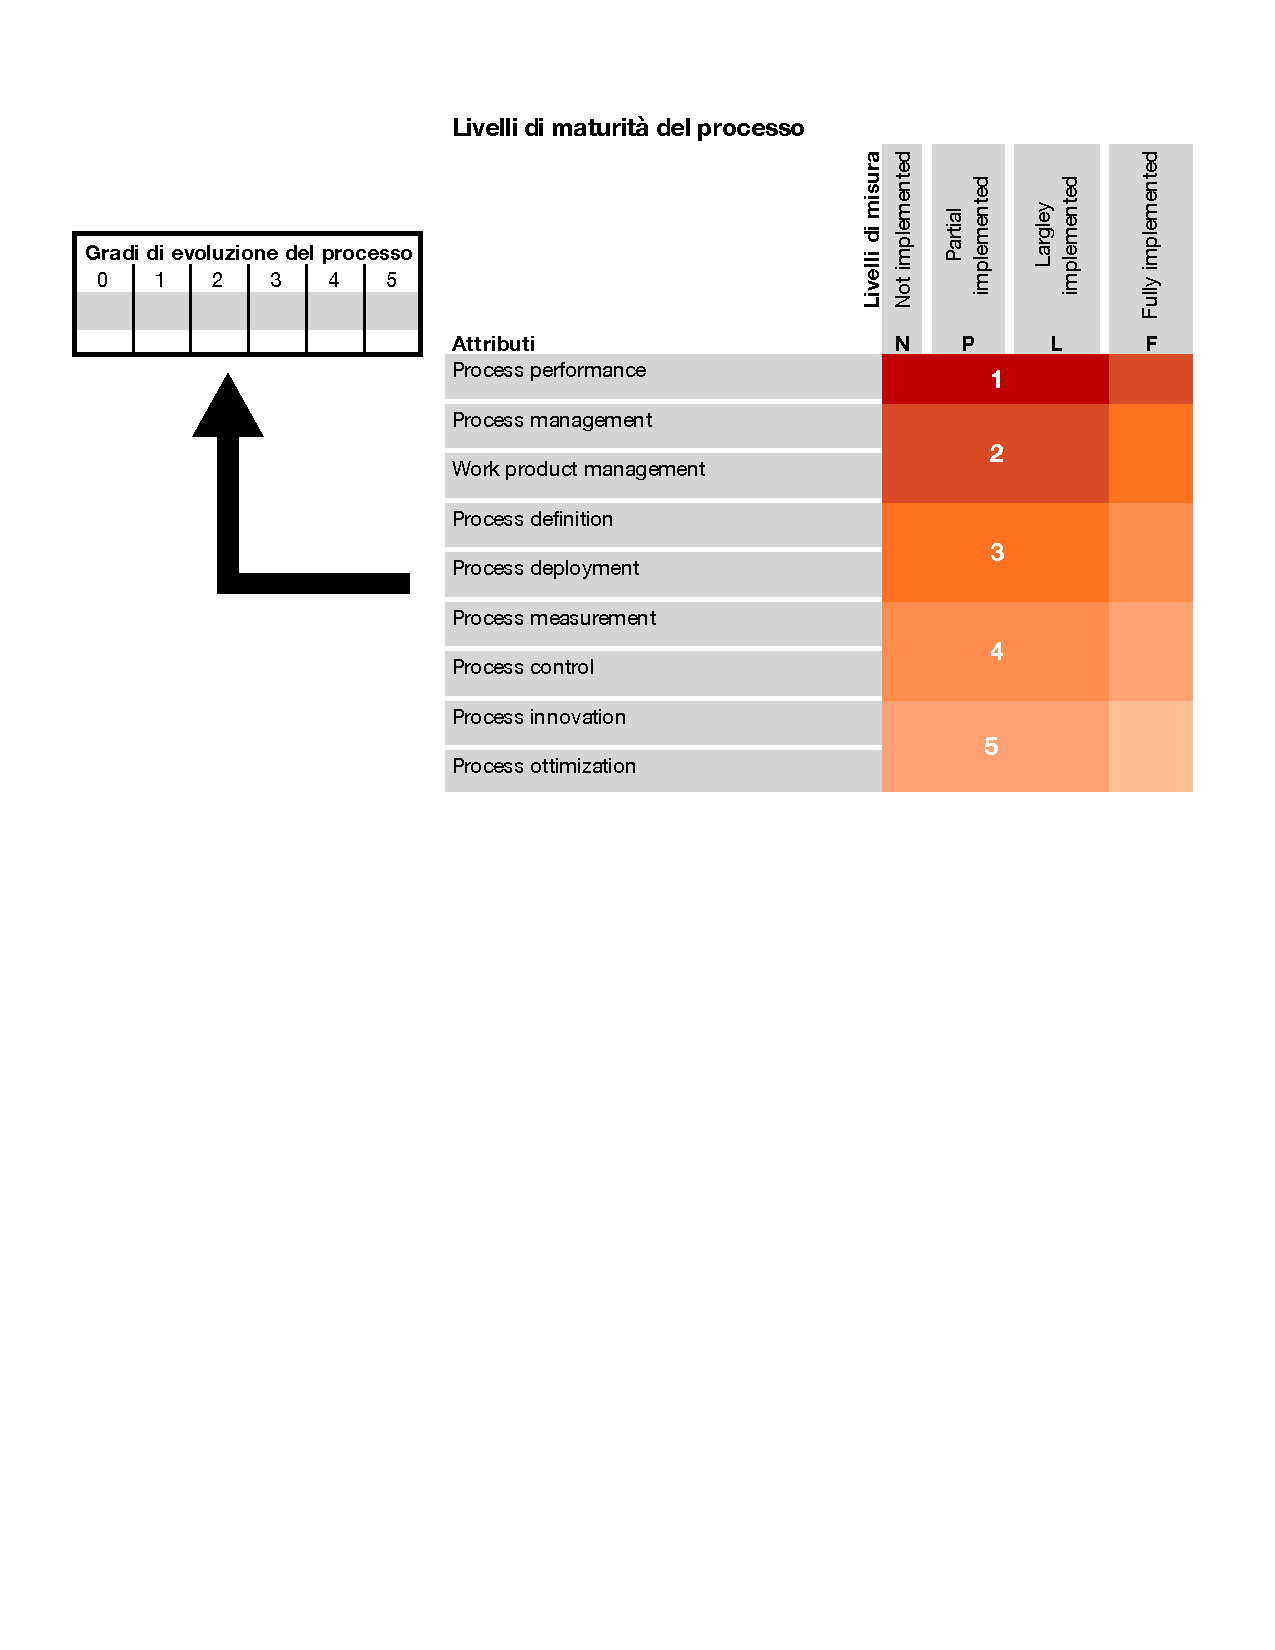
\includegraphics[scale=0.7]{images/ISOIEC15504.pdf}
	\caption{Riepilogo modello ISO/IEC 15504}
\end{figure}
\newpage

\subsection{Ciclo di Deming}
Il ciclo di Deming, noto anche come PDCA (dall'inglese \textbf{P}lan-\textbf{D}o-\textbf{C}heck-\textbf{A}ct), è un metodo di gestione iterativo suddiviso in quattro stadi ed utilizzato per il controllo del miglioramento continuo dei processi e dei prodotti. Esso permette, nello specifico, di migliorare gradualmente la qualità dei processi in termini di efficienza ed efficacia, ottimizzando l'uso delle risorse e misurando la loro conformità rispetto le aspettative. \\
La seguente immagine riporta le attività previste a tale scopo e ne segue una breve descrizione. 
\begin{figure}[htbp]
	\centering
	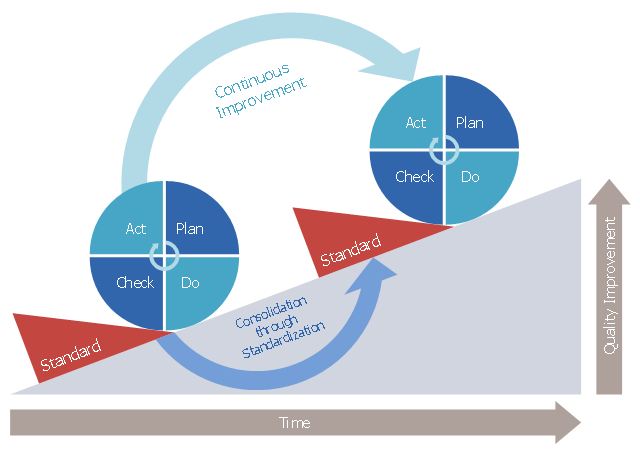
\includegraphics[scale=0.5]{images/pdca.png}
	\caption{Principio del miglioramento continuo secondo PDCA}
	
\end{figure}

\begin{itemize}
	\item \textbf{Plan}: prevede la definizione delle attività, scadenze, responsabilità e risorse atti a raggiungere e soddisfare degli obiettivi di miglioramento;
	\item \textbf{Do}: prevede l'esecuzione delle attività pianificate durante il periodo di pianificazione;
	\item \textbf{Check}: prevede la verifica dell'esito del processo in seguito all'attuazione delle strategie di miglioramento ed il confronto tra i risultati raccolti durante la fase Do e quelli attesi (specificati nella fase Plan) per stimare l'impatto effettivo del o dei miglioramenti apportati;
	\item \textbf{Act}: prevede l'attuazione delle strategie che hanno portato a dei miglioramenti. Nel caso i risultati attuali si distacchino da quelli previsti, si possono compiere delle azioni di correzione in seguito ad un'approfondita analisi delle cause di tale errore. 
\end{itemize}

\newpage
\section{ISO/IEC 9126}
Lo standard ISO/IEC 9126 definisce un modello dei requisiti qualitativi del Prodotto.
Il modello descritto si concentra in primo luogo sui tre punti di vista della qualità che esistono sul prodotto:
\begin{itemize}
	\item \textbf{Qualità esterna:} esprime il comportamento dinamico del software, in un determinato ambiente d'uso. In sostanza consiste nelle prestazioni e nelle funzionalità che il prodotto offre quando è in esecuzione;
	\item \textbf{Qualità interna:} esprime le proprietà statiche, cioè
	indipendenti dal contesto di esecuzione e uso. Sono direttamente misurabili ad esempio sul
	codice sorgente, pertanto senza la necessità di eseguire il software;
	\item \textbf{Qualità in uso:} esprime il livello con cui il prodotto si dimostra utile all'utente nel suo contesto d'uso. In altre parole rappresenta la capacità del prodotto di dare efficacia ed efficienza al lavoro dell'utente, a fronte di una sicurezza di utilizzo e di una soddisfazione nel far uso del prodotto.
\end{itemize}
\subsection{Modello per la qualità esterna ed interna}
Per la qualità esterna ed interna è definito un modello gerarchico formato da 6 caratteristiche principali e numerose sottocaratteristiche, tutte misurabili direttamente o indirettamente grazie all'utilizzo di metriche.
Le sei caratteristiche principali sono elencate di seguito:
\begin{itemize}
	\item \textbf{Funzionalità:} rappresenta la capacità del prodotto software di fornire funzioni che soddisfano le esigenze stabilite, sia esplicite che implicite, quando il software opera in un determinato contesto di utilizzo. Sottocaratteristiche notevoli sono l'interoperabilità e la Sicurezza, intesa come la capacità di proteggere le informazioni e i dati da accessi non autorizzati;
	\item \textbf{Affidabilità:} capacità di mantenere uno specificato livello di prestazione quando si opera in specificate condizioni. Sottocaratteristiche importanti sono la maturità e la tolleranza all'errore;
	\item \textbf{Efficienza:} capacità di fornire le funzioni richieste nel minor tempo possibile, sfruttando al meglio le risorse messe a disposizione;
	\item \textbf{Usabilità:} capacità del prodotto software di essere capito, appreso, usato e gradito all'utente, quando usato in contesti specificati. Una sottocaratteristica di rilievo è l'attrattiva;
	\item \textbf{Manutenibilità:} capacità del software di essere modificato e manutenuto. Per modifiche si intendono correzioni o adattamenti del software, negli ambienti, nei requisiti e nelle specifiche funzionali. Una sottocaratteristica importante è la testabilità, cioè la capacità di un software di consentire la verifica e di essere oggetto di test;
	\item \textbf{Portabilità:} capacità di poter essere trasferito da un ambiente di esecuzione all'altro.
\end{itemize}
\subsection{Modello per la qualità in uso}
Per la qualità in uso lo standard definisce una gerarchia separata, per enfatizzare il fatto che qui si considera non solo il prodotto software in sè, ma la relazione stretta tra esso e l'utente, nell'ambiente di utilizzo. Il modello è formato dalle seguenti quattro caratteristiche:
\begin{itemize}
	\item \textbf{Efficacia:} rappresenta la capacità di supportare un utente nel raggiungere i suoi obiettivi con accuratezza e completezza in un dato contesto;
	\item \textbf{Produttività:} la capacità di supportare un utente nello spendere l’appropriata quantità di risorse in relazione all’efficacia dei risultati da raggiungere; 
	\item \textbf{Soddisfazione:} la capacità di soddisfare un utente in un dato contesto d’uso;
	\item \textbf{Safety:} la capacità di raggiungere accettabili livelli di rischio di
	danni a persone, al software, ad apparecchiature, o all’ambiente operativo in un dato contesto d’uso.
\end{itemize}
\begin{figure}[htbp]
	\centering
	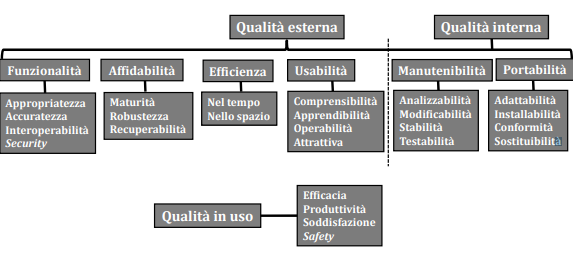
\includegraphics{images/gerarchiaQualitaProdotto.png}
	\caption{Riepilogo modello ISO 9126}
\end{figure}